%input macros (i.e. write your own macros file called MacroFile1.tex)
\newcommand{\PdfPsText}[2]{
  \ifpdf
     #1
  \else
     #2
  \fi
}

\newcommand{\IncludeGraphicsH}[3]{
  \PdfPsText{\includegraphics[height=#2]{#1}}{\includegraphics[bb = #3, height=#2]{#1}}
}

\newcommand{\IncludeGraphicsW}[3]{
  \PdfPsText{\includegraphics[width=#2]{#1}}{\includegraphics[bb = #3, width=#2]{#1}}
}

\newcommand{\InsertFig}[3]{
  \begin{figure}[!htbp]
    \begin{center}
      \leavevmode
      #1
      \caption{#2}
      \label{#3}
    \end{center}
  \end{figure}
}


%%% Local Variables: 
%%% mode: latex
%%% TeX-master: "~/Documents/LaTeX/CUEDThesisPSnPDF/thesis"
%%% End: 

\documentclass[report,12pt]{Classes/CUEDthesisPSnPDF}
\usepackage{amsmath}
\usepackage{multirow}
\usepackage{layouts}
\usepackage{array}
\allowdisplaybreaks
\ifpdf
    \pdfinfo { /Title  (Thesis)
               /Creator (TeX)
               /Producer (pdfTeX)
               /Author (Nikolaos Kofinas nikofinas@gmail.com)
               /CreationDate (D:20120619000000)  %format D:YYYYMMDDhhmmss
               /ModDate (D:20120619000000)
               /Subject ()
               /Keywords (Robocup, Kouretes,Kinematics,Nao,Kofinas,Inverse, Thesis)}
    \pdfcatalog { /PageMode (/UseOutlines)
                  /OpenAction (fitbh)  }
\fi

\title{{\LARGE Forward and Inverse Kinematics\\for the Nao Humanoid Robot}}%\\Cartesian control of robot joints}
\ifpdf
  \author{Nikolaos Kofinas}
  \collegeordept{\href{http://www.ece.tuc.gr}{Department of Electronic and Computer Engineering}}
  \university{\href{http://www.tuc.gr}{Technical University of Crete, Greece}}
  \crest{
\includegraphics[height=40mm]{Figures/TUClogocolor.jpg}}
\else
  \author{Nikolaos Kofinas}
  \collegeordept{Department of Electronic and Computer Engineering}
  \university{Technical University of Crete, Greece}
  \crest{
\includegraphics[height=40mm]{Figures/TUClogocolor.jpg}}
\fi

\committee{
\begin{normalsize}Thesis Committee\end{normalsize}\\
Assistant Professor Michail G. Lagoudakis (ECE)\\
Professor Minos Garofalakis (ECE)\\
Assistant Professor Aggelos Bletsas (ECE)
}
\degreedate{Chania, Jule 2012}

\rfoot{July 2012}
\cfoot{\thepage}
\lfoot{Nikolaos Kofinas}


% turn of those nasty overfull and underfull hboxes
\hbadness=10000
\hfuzz=50pt

\usepackage{fancyvrb}
\DefineVerbatimEnvironment{code}{Verbatim}{fontsize=\small}
\DefineVerbatimEnvironment{example}{Verbatim}{fontsize=\small}

\usepackage{subfigure}

% Put all the style files you want in the directory StyleFiles and usepackage like this:
%\usepackage{StyleFiles/watermark}

\begin{document}

%\language{english}
\en

 \renewcommand\baselinestretch{1.2}
\baselineskip=18pt plus1pt

% A page with the abstract on including title and author etc may be
% required to be handed in separately. If this is not so, then comment
% the below 3 lines (between '\begin{abstractseparte}' and 
% 'end{abstractseparate}'), normally like a declaration ... needs some more
% work, mind as environment abstracts creates a new page!
% \begin{abstractseparate}
%   
% Thesis Abstract -----------------------------------------------------

\begin{abstractslong}        %this creates the heading for the abstract page
Articulated robots with multiple degrees of freedom, such as humanoid robots, have become popular research platforms in robotics and artificial intelligence. Such robots can perform complex motions, including the balancing, walking, and kicking skills required in the RoboCup robot soccer competition. The design of complex dynamic motions is achievable only through the use of robot kinematics, which is an application of geometry to the study of arbitrary robotic chains. This thesis studies the problems of forward and inverse kinematics for the Aldebaran NAO humanoid robot and presents for the first time a complete analytical solution to both problems with no approximations, including an implementation of a software library for real-time execution. The forward kinematics allow NAO developers to map any configuration of the robot from its own joint space to the three-dimensional physical space, whereas the inverse kinematics provide closed-form solutions to finding joint configurations that drive the end effectors of the robot to desired points in the three-dimensional space. The proposed solution was made feasible through a decomposition into five independent problems (head, two arms, two legs), the use of the Denavit-Hartenberg method, and the analytical solution of a non-linear system of equations. The main advantage of the proposed inverse kinematics compared to existing numerical approaches is its accuracy, its efficiency, and the elimination of singularities. The implemented NAO kinematics library has been integrated into the software architecture of the RoboCup team ``Kouretes'' and is currently being used in various motion design problems, such as center-of-mass calculation, balancing, trajectory following, dynamic kicking, and omnidirectional walking. 




\end{abstractslong}
\newpage
\ 


 \begin{abstractsgreeklong}
{\gr 
�� ������� ������ �� ���������� ������� ����������, ���� �� ����������� ������, ����� ����� ���������� ���������� ������� ��� ��������� ��� ��� ������� ���������. �� �� ���� ������ ������� �� ���������� �������� ��������, ������������������� ��� ��� ���������� ����������, ���������� ��� ����������� ��� ����������� ���� ���������� ���������� ����������� {\en RoboCup}. � ���������� ���������� ��������� �������� ������ �� ���������� ���� ���� ��� ������ ���������� �����������, ��� ����� � �������� ��� ���������� ��� ������ ���������� ���������� ��������. � ������� ����������� ������� ������ �� ���������� ��� ������� ��� ����������� ����������� ��� �� ������������ ������ {\en Aldebaran NAO} ��� ����������� ��� ����� ���� ��� ����� ��������� ���� ��� ��� �� ��� ���������� ����� ������������, ������������������� ���� ���������� ����������� ���������� ��� �������� �� ���������� �����. � ������ ���������� ��������� ����� ��������������� ��� ��� �� ������������ ����������� ������� ��� ������ ��� ��� ���� ��� ��������� ��� ���� ������������ ������ ����, ��� � ���������� ���������� ������� ������ �������� ������ ��� ��� �������� ��������� ��� ��������� ��� ������� �� ���� ��� ������ �� ��������� ������ ���� ������������ ����. � ������������ ���� ������� ������ ���� ���� ���������� �� ����� ���������� ���������� (������, ��� �����, ��� �����), ��� ����� ��� ������� {\en Denavit-Hartenberg} ��� ���� ��������� ������� ���� ��-��������� ���������� ���������. �� ����� ����������� ��� ������������� ����������� ����������� �� �������� �� ����������� ����������� ������������ ����� � �������� ���, � ������������� ��� ��� � �������� ��� ���������� �����������. � ����������� ���������� ����������� ��� �� ��� ���� ����������� ���� ������������� ���������� ��� ������ {\en RoboCup} ((��������)) ��� ��������������� �� ������� ���������� ���������� ��������, ���� ����������� ��� ������� �����, ���������, ������������� �������, �������� ���������� ��� ���������������� �������.
}
 \end{abstractsgreeklong}

\newpage
\ 


% ----------------------------------------------------------------------


%%% Local Variables: 
%%% mode: latex
%%% TeX-master: "../thesis"
%%% End: 

% \end{abstractseparate}



% Using the watermark package which is in StyleFiles/
% and to remove DRAFT COPY ONLY appearing on the top of all pages comment out below line
%\watermark{DRAFT COPY ONLY}

 % English Title Page
\maketitle
    \cleardoublepage
 % Greek Title Page
 {\gr
     \thispagestyle{empty}
  \begin{center}
    \setlength{\parskip}{0pt}
    {\large \sc {\href{http://www.tuc.gr}{����������� ������}} \par}
      \vspace*{1ex}
    {\large \sc {\href{http://www.ece.tuc.gr}{�����}} \par}
      \vspace*{20mm}
    { \Large {\bfseries {{\LARGE \gr �thema Nao}}} \par}
	{\large \vspace*{10mm} {
\includegraphics[height=40mm]{Figures/TUClogocolor.jpg} \par} \vspace*{15mm}}	
    {{\Large �������� �������} \par}
	\vspace*{15mm}
    {\large {\begin{normalsize}epitropi\end{normalsize}\\
epitropi1\\
epitropi2\\
epitropi3} \par}
	\vfill
    {\large xania ioulios 2012}
  \end{center}
  \null\vfill
}
    \cleardoublepage

%set the number of sectioning levels that get number and appear in the contents
\setcounter{secnumdepth}{3}
\setcounter{tocdepth}{2}

\frontmatter
 First of all, I would like to thank Manolis Orf (a.k.a. ``re palikari'') for his help and the great ideas as well as the great fights. \\
Next I would like to thank my professor Michail G. Lagoudakis, for the inspiration and the trust that he showed to me.\\
Fanoula is the next person that I would like to thank:). She helped me so much during this difficult period and I am so o lucky that she still talks to me.\\
Team Kouretes,(N.Pav, A.Top, M.Kounoupidi, D.Janetatou, Orf) I can't understand why you talk to me after all the things we've been through together in ``ypoga''. Finally, I like this team and our lab more than that I had imagined, thank you for the help and the fun team.\\
To sum up, I would like to thank my friends, with whom I had the greatest five years of my life. N. Pavlakis (he paid five Euro for the second reference), E.Alimpertis, K.Perros and E.Soulas, thank you for everything.\\
Of course, I don't have words to describe the help from my parents, so I ....
% ----------------------------------------------------------------------


%%% Local Variables: 
%%% mode: latex
%%% TeX-master: "../thesis"
%%% End: 

 
% Thesis Abstract -----------------------------------------------------

\begin{abstractslong}        %this creates the heading for the abstract page
Articulated robots with multiple degrees of freedom, such as humanoid robots, have become popular research platforms in robotics and artificial intelligence. Such robots can perform complex motions, including the balancing, walking, and kicking skills required in the RoboCup robot soccer competition. The design of complex dynamic motions is achievable only through the use of robot kinematics, which is an application of geometry to the study of arbitrary robotic chains. This thesis studies the problems of forward and inverse kinematics for the Aldebaran NAO humanoid robot and presents for the first time a complete analytical solution to both problems with no approximations, including an implementation of a software library for real-time execution. The forward kinematics allow NAO developers to map any configuration of the robot from its own joint space to the three-dimensional physical space, whereas the inverse kinematics provide closed-form solutions to finding joint configurations that drive the end effectors of the robot to desired points in the three-dimensional space. The proposed solution was made feasible through a decomposition into five independent problems (head, two arms, two legs), the use of the Denavit-Hartenberg method, and the analytical solution of a non-linear system of equations. The main advantage of the proposed inverse kinematics compared to existing numerical approaches is its accuracy, its efficiency, and the elimination of singularities. The implemented NAO kinematics library has been integrated into the software architecture of the RoboCup team ``Kouretes'' and is currently being used in various motion design problems, such as center-of-mass calculation, balancing, trajectory following, dynamic kicking, and omnidirectional walking. 




\end{abstractslong}
\newpage
\ 


 \begin{abstractsgreeklong}
{\gr 
�� ������� ������ �� ���������� ������� ����������, ���� �� ����������� ������, ����� ����� ���������� ���������� ������� ��� ��������� ��� ��� ������� ���������. �� �� ���� ������ ������� �� ���������� �������� ��������, ������������������� ��� ��� ���������� ����������, ���������� ��� ����������� ��� ����������� ���� ���������� ���������� ����������� {\en RoboCup}. � ���������� ���������� ��������� �������� ������ �� ���������� ���� ���� ��� ������ ���������� �����������, ��� ����� � �������� ��� ���������� ��� ������ ���������� ���������� ��������. � ������� ����������� ������� ������ �� ���������� ��� ������� ��� ����������� ����������� ��� �� ������������ ������ {\en Aldebaran NAO} ��� ����������� ��� ����� ���� ��� ����� ��������� ���� ��� ��� �� ��� ���������� ����� ������������, ������������������� ���� ���������� ����������� ���������� ��� �������� �� ���������� �����. � ������ ���������� ��������� ����� ��������������� ��� ��� �� ������������ ����������� ������� ��� ������ ��� ��� ���� ��� ��������� ��� ���� ������������ ������ ����, ��� � ���������� ���������� ������� ������ �������� ������ ��� ��� �������� ��������� ��� ��������� ��� ������� �� ���� ��� ������ �� ��������� ������ ���� ������������ ����. � ������������ ���� ������� ������ ���� ���� ���������� �� ����� ���������� ���������� (������, ��� �����, ��� �����), ��� ����� ��� ������� {\en Denavit-Hartenberg} ��� ���� ��������� ������� ���� ��-��������� ���������� ���������. �� ����� ����������� ��� ������������� ����������� ����������� �� �������� �� ����������� ����������� ������������ ����� � �������� ���, � ������������� ��� ��� � �������� ��� ���������� �����������. � ����������� ���������� ����������� ��� �� ��� ���� ����������� ���� ������������� ���������� ��� ������ {\en RoboCup} ((��������)) ��� ��������������� �� ������� ���������� ���������� ��������, ���� ����������� ��� ������� �����, ���������, ������������� �������, �������� ���������� ��� ���������������� �������.
}
 \end{abstractsgreeklong}

\newpage
\ 


% ----------------------------------------------------------------------


%%% Local Variables: 
%%% mode: latex
%%% TeX-master: "../thesis"
%%% End: 


\tableofcontents
\listoffigures
%\printglossary  %% Print the nomenclature
%\addcontentsline{toc}{chapter}{Nomenclature}


\mainmatter

 \chapter{Introduction}
\label{intro}
NAO is the robot that is used for the soccer games in RoboCup SPL league. In this league, all the teams are using the same robot and the same hardware, too. Thus, the teams need to implement their own omni-directional walk~\cite{naowalk}~\cite{bhumanwalk}, motions and balancing system if they want to be more competitive. The creation of dynamic movements, as the above, are not feasible without an inverse kinematics mechanism. Also, creation of a balancing system is impossible without the calculation of the center of mass using forward kinematics. This mechanism must be fast, because the RoboCup is a real-time environment. This thesis describes a forward kinematics solution for every chain of NAO and an analytical solution for the problem of inverse kinematics without any approximations.

\section{Thesis Contribution}
As it mentioned before, there is a need to know the position of an end effector and the execution of dynamic trajectories. With this thesis we succeeded to implement the mechanism that translates the joints of a chain to a Cartesian position for the end effector. Also, we created a mechanism that translates dynamic trajectories to joint values in real execution time. The contribution of this thesis to our SPL team, Kouretes, is the mechanism of inverse kinematics that makes possible the creation of our own omni-directional walk and kick engine.

\section{Thesis Outline}
Chapter~\ref{Background} describes the RoboCup competition, the Standard Platform League (SPL), our SPL team Kouretes, and the Aldebaran NAO humanoid robot. Furthermore, it provides basic background information about  generic robot kinematics, affine transformation matrices, and the Denavit-Hartenberg (DH) parameters. In Chapter~\ref{problem} we provide a complete description of the NAO hardware and we define the problem of kinematics for the NAO robot. Moreover, in Chapter~\ref{related} we discuss the related work about forward and mainly inverse kinematics for the NAO robot. In Chapter~\ref{approach} we describe in detail our solutions to the problems of forward and inverse kinematics for the NAO robot. Additionally, we explain the implementation of kinematics and integration with our team's code. In Chapter~\ref{Results} we present the real-time performance of our kinematics mechanism and a couple of scenarios to demonstrate its effectiveness. Finally, in Chapter~\ref{conclusion} we discuss the results of this thesis and we compare it with other related approaches, pointing out at the same time possible future directions.


 \chapter{Background}
\label{Background}
\section{RoboCup}
The RoboCup competition was initially inspired by Hiroaki Kitano~\cite{robocup} in 1993 and his idea eventually led to the establishment of the RoboCup Federation. The RoboCup competition has a bold vision: ``By the year 2050, to develop a team of fully autonomous humanoid robots that can win against the human world soccer champions''. All the teams participating in RoboCup have to find real-time solutions to some of the most difficult problems in robotics (perception, cognition, action, coordination). All the divisions in RoboCup (soccer, RoboCup@Home, RoboRescue, etc.) are designed so as to test the proposed solutions by the various teams to the problems mentioned above. So far, the researchers participating in RoboCup have made a lot of progress in solving real-world problems that show up in the various RoboCup leagues within each division.

\subsection{Standard Platform League}
The Standard Platform League (SPL) is one of the many leagues in the soccer division of RoboCup. In this league all the teams use the same robot, the Aldebaran NAO humanoid robot, and they focus only on algorithm design and software development for this robot. For this reason, the teams are prohibited to make any changes to the hardware of the robot. The robots are completely autonomous and no human intervention from team members is allowed during the games. The only interaction of the robots with the ``outer world'' is the reception of data from the Game Controller, a computer that broadcasts information about the state of the game (score, time, penalties, etc.).

\begin{figure}[t!]
	\begin{center}
		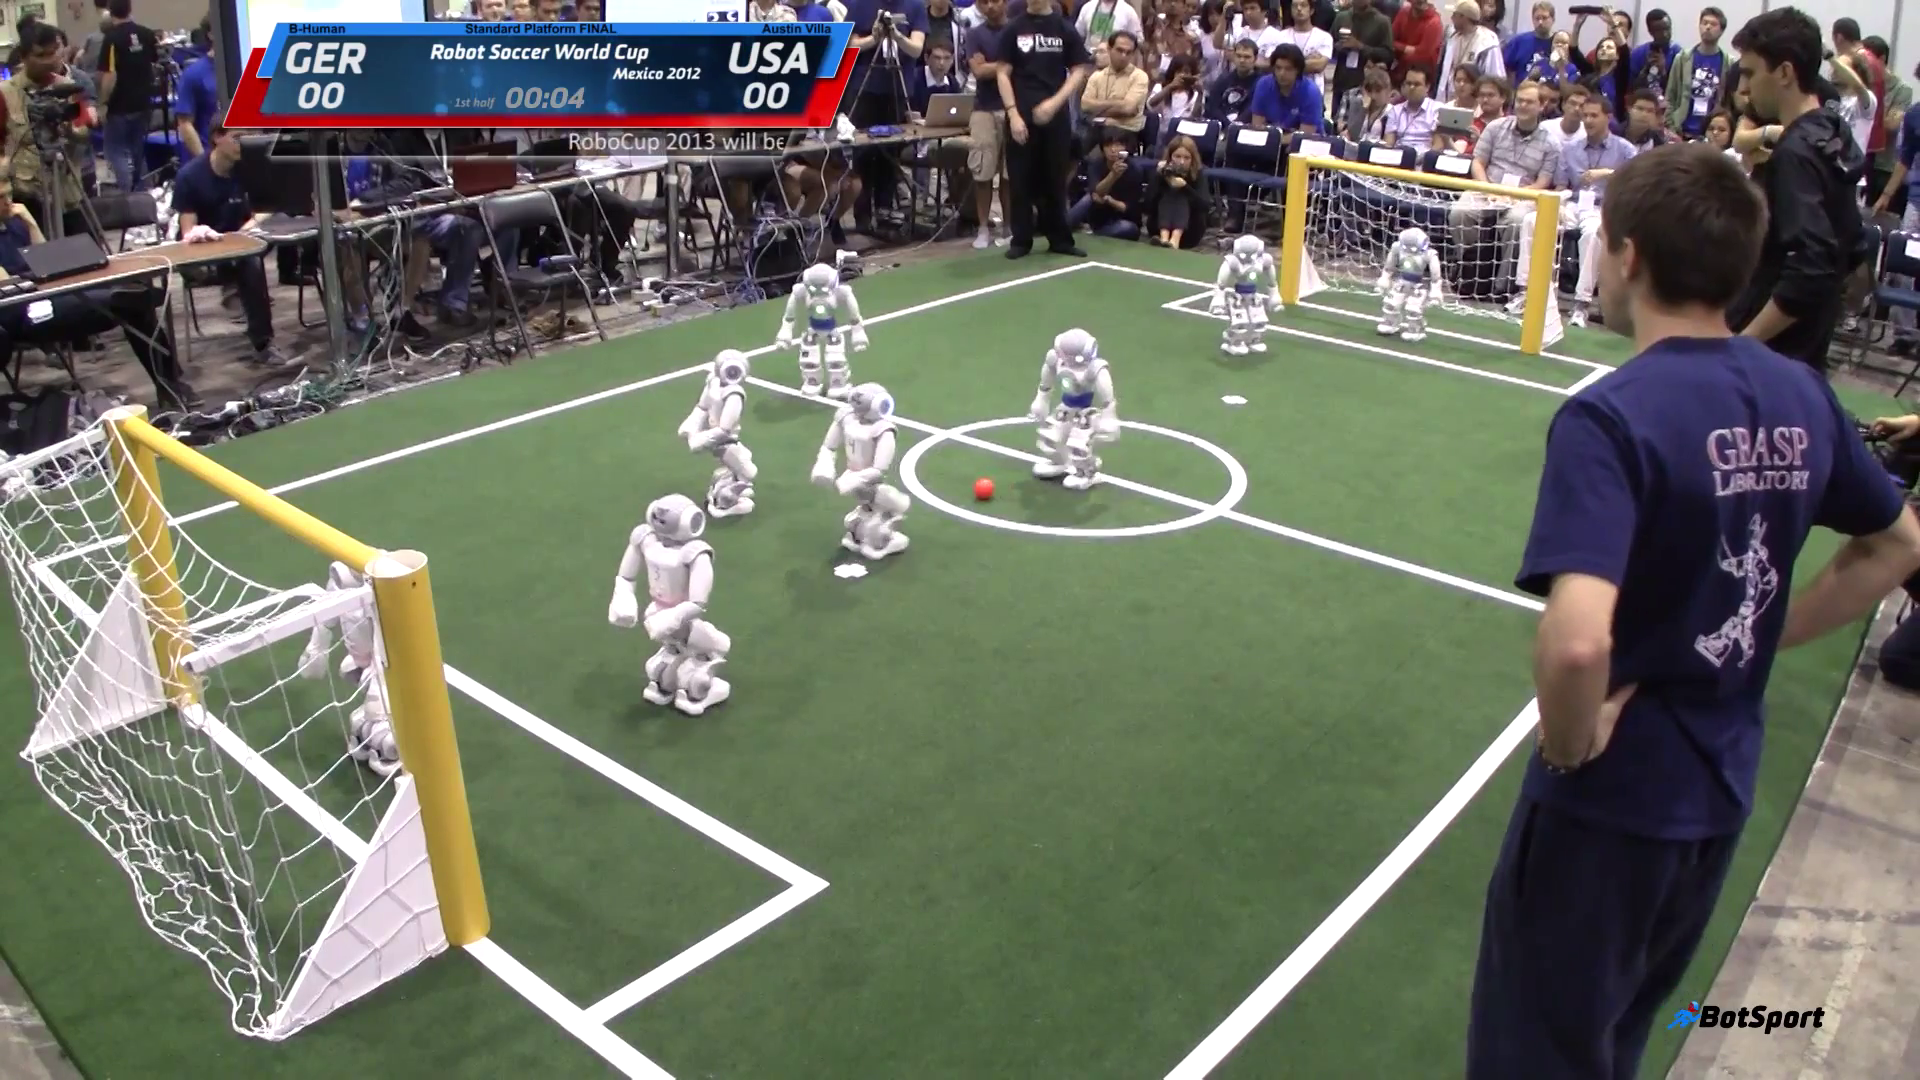
\includegraphics[width=.9\textwidth]{Figures/spl2012.png}
 		\caption{Standard Platform League at RoboCup 2012 (from \url{www.botsport.tv})}
 		\label{fig:RoboCup SPL}
	\end{center}
\end{figure}

Currently, the SPL games are conducted on a field with dimensions $4m \times 6m$~\cite{SPLrules2012}. The field consists of a green carpet marked with white lines and two yellow goals (Figure~\ref{fig:RoboCup SPL}). The appearance of the field is similar to a real soccer field, but it is scaled to the size of the robots. The ball is an orange street hockey ball. Each team consists of four robots and each robot carries a colored waist band (blue or pink) that distinguishes the teams. The total game time is 20 minutes and is broken in two halves; each half lasts 10 minutes.




\begin{figure}[t!]
	\begin{center}
		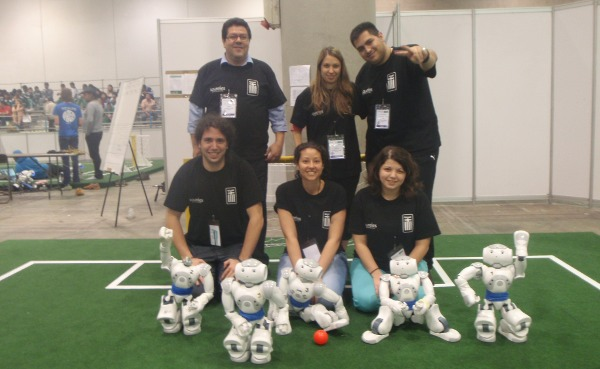
\includegraphics[width=.9\textwidth]{Figures/robocup2012-team.jpg}
 		\caption{Team Kouretes at RoboCup 2012 in Mexico City}
 		\label{fig:Kouretes2012}
	\end{center}
\end{figure}

\section{Robocup SPL Team Kouretes}

Team Kouretes (\url{www.kouretes.gr}) is the RoboCup team of the Technical University of Crete. The team was founded in 2006 and participates in the main RoboCup competition ever since in various leagues (Four-Legged, Standard Platform, MSRS, Webots), as well as in various local RoboCup events (German Open, Mediterranean Open, Iran Open, RC4EW, RomeCup) and RoboCup exhibitions (Athens Digital Week, Micropolis, Schoolfest). In May 2010, the team hosted the 1st official SPL tournament in Greece (with three invited teams) within the Hellenic Conference on Artificial Intelligence (SETN). Distinctions of the team include: {\bf 2nd} place in MSRS at RoboCup 2007; {\bf 3rd} place in SPL-Nao, {\bf 1st} place in SPL-MSRS, among the {\bf top 8} teams in SPL-Webots at RoboCup 2008; {\bf 1st} place in RomeCup 2009; {\bf 6th} place in SPL-Webots at RoboCup 2009; {\bf 2nd} place in SPL at RC4EW 2010; and {\bf 2nd} place in SPL Open Challenge Competition at RoboCup 2011 (joint team Noxious-Kouretes).

The team has been developing its own (publicly-available) software for the Nao robots since 2008. The team code repository includes a custom software architecture, a custom communication framework, graphical tools for monitoring and behavior specification, and modules for object recognition, state estimation, localization, obstacle avoidance, behavior execution, team coordination. The members of the team are senior undergraduate ECE students working on their diploma thesis on a RoboCup-related topic; 15 diploma theses have been completed so far. Recently, the team participated in the RoboCup German Open 2012 competition in Magdeburg, in RoboCup Iran Open 2012 in Tehran, and in RoboCup 2012 in Mexico City (Figure~\ref{fig:Kouretes2012}). In the most recent RoboCup 2012 competition, the team succeeded to proceed to the second round-robin round and rank among the top-16 SPL teams in the world.

\section{Aldebaran NAO Humanoid Robot}
NAO is an integrated, programmable, medium-sized humanoid robot developed by Aldebaran Robotics in Paris, France~\cite{naopaper}. Project NAO started in 2004. In August 2007 NAO officially replaced Sony's AIBO quadruped robot in the RoboCup SPL. In the past few years NAO has evolved over several designs and several versions. 

\begin{figure}[t!]
	\begin{center}
		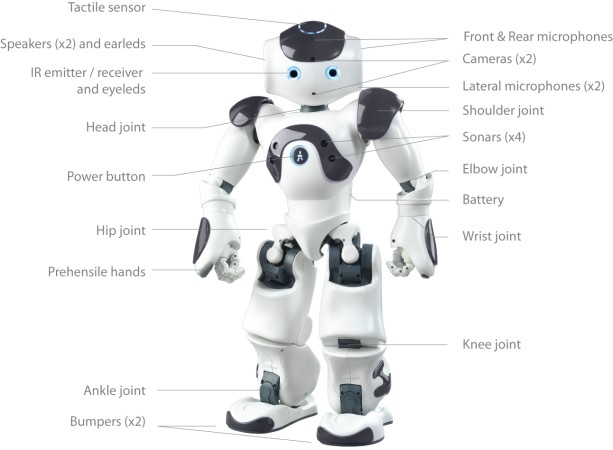
\includegraphics[height = 8cm]{Figures/nao.jpg}
 		\caption{Components of NAO v3.3}
 		\label{fig:sensors}
	\end{center}
\end{figure}

NAO (version V3.3) is a 58cm, 5kg humanoid robot (Figure~\ref{fig:sensors}). The NAO robot carries a fully capable computer on-board with an x86 AMD Geode processor at 500 MHz, 256 MB SDRAM, and 2 GB flash memory running an Embedded Linux distribution. It is powered by a 6-cell Lithium-Ion battery which provides about 30 minutes of continuous operation and communicates with remote computers via an IEEE 802.11g wireless or a wired ethernet link. 

NAO RoboCup edition has 21 degrees of freedom; 2 in the head, 4 in each arm, 5 in each leg and 1 in the pelvis (there are two pelvis joints which are coupled together on one servo and cannot move independently). NAO, also, features a variety of sensors. Two cameras are mounted on the head in vertical alignment providing non-overlapping views of the lower and distant frontal areas, but only one is active each time and the view can be switched from one to the other almost instantaneously. Each camera is a $640 \times 480$ VGA devise operating at 30fps. Four sonars (two emitters and two receivers) on the chest allow NAO to sense obstacles in front of it. In addition, the NAO has a rich inertial unit, with one 2-axis gyroscope and one 3-axis accelerometer, in the torso that provides real-time information about its instantaneous body movements. Two bumpers located at the tip of each foot are simple ON/OFF switches and can provide information on collisions of the feet with obstacles. Finally, an array of force sensitive resistors on each foot delivers feedback of the forces applied to the feet, while encoders on all servos record the actual positions of all joints at each time.



\section{Robot Kinematics}
A \textit{robot kinematic chain} is an articulated manipulator that interacts with the environment and is typically described as an assembly of robotic links connected by (rotary) joints. The joints rotate and control the relative angular positioning of the links of the manipulator. Not all combinations of joints' positions in the chain are valid, because some combinations lead to collisions between the links of the chain or with some fixed item of the environment, such as the floor or a wall. All the valid combinations of joint positions form the \textit{joint space}. The term \textit{degrees of freedom} (DOF) refers to the number of joints in a kinematic chain; clearly, more DOFs imply more flexibility in the motion of the chain. 

\textit{Robot kinematics} is the application of geometry to the study of  kinematic chains with multiple degrees of freedom. More specifically, robot kinematics provide the transformation from the joint space, where the kinematic chains are defined, to the Cartesian space, where the robot manipulator moves, and vice versa. Robot kinematics are quite useful, because they can be used for planning and executing movements, as well as calculating actuator forces and torques.



\subsection{Forward Kinematics}
The joint space reveals very little information about the position of the end effector of the kinematic chain. The \textit{forward kinematics} define a mapping from the joint space to the three-dimensional Cartesian space. Given a kinematic chain with $m$ joints and a set of joint values $(\theta_1, \theta_2,\ldots,\theta_m)$, the forward kinematics can find the point $(p_x,p_y,p_z)$ and the orientation $(a_x,a_y,a_z)$ of the end effector of the kinematic chain in the three-dimensional $x$-$y$-$z$ space. Forward kinematics is a domain-independent problem and can be solved for any simple or complex kinematic chain yielding a closed-form, analytical solution. 

\subsection{Inverse Kinematics}
Robot manipulators typically need to reach target points or follow trajectories in the three-dimensional space. To make the end effector reach a point or follow a trajectory, one has to specify appropriate values for the joints of the kinematic chain. The \textit{inverse kinematics} define ways to go from the three-dimensional space to the joint space. In particular, the inverse kinematics define a relation between positions in the three-dimensional space (point $(p_x,p_y,p_z)$ and orientation $(a_x,a_y,a_z)$) and joint values/angles $(\theta_1, \theta_2,\ldots,\theta_m)$ in the joint space of a kinematic chain with $m$ joints. The problem of inverse kinematics is domain-dependent and every kinematic chain has a different solution. The solution to the inverse kinematics problem can lead to an analytical, closed-form equation or to a numerical, iterative approximation (e.g. with the Jacobian approximation method). As the DOFs increase, a point in the three-dimensional space may have more than one matching point in the joint space. This multiplicity of solutions makes the inverse kinematics a relation, not a mapping.




\section{Affine Transformations}
An affine transformation is a mapping that transforms points and vectors from one space to another, in a way that preserves the ratios of distances. The source and target spaces can be $n$-dimensional with $n\ge2$. The following are affine transformations: geometric contraction, expansion, dilation, reflection, rotation, shear, similarity transformations, spiral similarities, and translation. All the possible combinations of the above produce an affine transformation as well. The flexibility of affine transformations with respect to object representation in different spaces, makes it a very useful tool in computer graphics.

For the purposes of this thesis we only use rotation and translation, so we will focus only on these two types of affine transformation. Additionally, we are working in a three-dimensional Cartesian work space and therefore all the definitions and examples from now on will focus on this space.

\subsubsection*{Affine Transformation Matrix}
An affine transformation matrix is a $\big(\left(n+1\right)\times \left(n+1\right)\big)$ matrix, where $n$ is the number of dimensions in the space the transformation is defined on. In general, an affine transformation matrix is a block matrix of the form:
\[
T = 
\begin{bmatrix}
X & Y \\
\begin{bmatrix}
0 & \cdots & 0
\end{bmatrix} & 1
\end{bmatrix}
\]
where $X$ is a ($n\times n$) matrix, $Y$ is a ($n\times 1$) vector and the last line of $T$ contains $n-1$ zeros followed by a $1$. If we want to apply the transformation, to a given point  $p=(p_1,p_2,\ldots,p_n)$ in the $n$-dimensional space, we simply multiply the affine transformation matrix with the column vector $v=(p_1,p_2,\ldots,p_n,1)^\top$:
\[
v' = 
\begin{bmatrix}
p'_1\\
\vdots\\
p'_n\\
1
\end{bmatrix}
=
Tv = 
\begin{bmatrix}
X & Y \\
\begin{bmatrix}
0 & \cdots & 0
\end{bmatrix} & 1
\end{bmatrix}
\begin{bmatrix}
p_1\\
\vdots\\
p_n\\
1
\end{bmatrix}
\]
For a point  $p=(p_x,p_y,p_z)$ in the three-dimensional space, the transformation will be:
\[
v' = 
\begin{bmatrix}
p'_x\\
p'_y\\
p'_z\\
1
\end{bmatrix}
=
Tv = 
\begin{bmatrix}
X_{xx} & X_{xy} & X_{xz} & Y_x\\
X_{yx} & X_{yy} & X_{yz} & Y_y\\
X_{zx} & X_{zy} & X_{zz} & Y_z \\
0 & 0 & 0 & 1
\end{bmatrix} 
\begin{bmatrix}
p_x\\
p_y\\
p_z\\
1
\end{bmatrix}
\]
The matrix that results from the multiplication of two affine transformation matrices $T_1$ and $T_2$ is still an affine transformation:
\[
T = T_1 T_2 =
\begin{bmatrix}
X_1 & Y_1 \\
\begin{bmatrix}
0 & \cdots & 0
\end{bmatrix} & 1
\end{bmatrix}
\begin{bmatrix}
X_2 & Y_2 \\
\begin{bmatrix}
0 & \cdots & 0
\end{bmatrix} & 1
\end{bmatrix}
=
\begin{bmatrix}
X_1 X_2 & X_1Y_2+Y_1 \\
\begin{bmatrix}
0 & \cdots & 0
\end{bmatrix} & 1
\end{bmatrix}
\]
This property generalizes to the product of any number of affine transformation matrices:
\[
\widehat{T} = T_1 T_2 T_3 \cdots T_k = 
\begin{bmatrix}
\widehat{X} & \widehat{Y} \\
\begin{bmatrix}
0 & \cdots & 0
\end{bmatrix} & 1
\end{bmatrix}
\]
An affine transformation matrix is invertible, if and only if X is invertible, and takes the form:
\[
T^{-1} = 
\begin{bmatrix}
X^{-1} & -X^{-1}Y \\
\begin{bmatrix}
0 & \cdots & 0
\end{bmatrix} & 1
\end{bmatrix}
\]

\subsubsection*{Translation Matrix}

Translation in a Cartesian space is a function that moves (translates) every point by a fixed distance in a specified direction. We can describe a translation in the three-dimensional space with a ($4\times4$) matrix of the following form:
\[
A = 
\begin{bmatrix}
1 & 0 & 0 & d_x\\
0 & 1 & 0 & d_y\\
0 & 0 & 1 & d_z\\
0 & 0 & 0 & 1
\end{bmatrix}
\]
where $d_x$, $d_y$, and $d_z$ define the distance of translation along the $x$, $y$, and $z$ axis respectively. Apparently, the translation matrix is an affine transformation matrix with $X = I$. Therefore, to move a point $p=(p_x,p_y,p_z)$ in the three-dimensional space by distances $(d_x,d_y,d_z)$, we simply apply the transformation:
\[
v' = 
\begin{bmatrix}
p'_x\\
p'_y\\
p'_z\\
1
\end{bmatrix}
=
Av = 
\begin{bmatrix}
1 & 0 & 0 & d_x\\
0 & 1 & 0 & d_y\\
0 & 0 & 1 & d_z\\
0 & 0 & 0 & 1
\end{bmatrix}
\begin{bmatrix}
p_x\\
p_y\\
p_z\\
1
\end{bmatrix}
\]

\subsubsection*{Rotation Matrix}
Rotation in a Cartesian space is a function that rotates vectors by a fixed angle about a specified direction. A rotation in the $n$-dimensional space is described as an $(n\times n)$ orthogonal matrix $R$ with determinant 1:
\[
R^\top = R^{-1} \quad \quad  \quad
RR^\top = R^\top R = I \quad \quad  \quad
\det(R) = 1
\]
In the three-dimensional Cartesian space there are three distinct rotation matrices, each one of them performing a rotation of $\theta_x$, $\theta_y$, $\theta_z$ about the $x$, $y$, $z$ axis respectively, assuming a right-handed coordinate system:
\[
R_x = 
\begin{bmatrix}
1 & 0 & 0 \\
0 & \cos\theta_x & -\sin\theta_x \\
0 & \sin\theta_x & \cos\theta_x
\end{bmatrix}
\quad
R_y = 
\begin{bmatrix}
\cos\theta_y & 0 & \sin\theta_y \\
0 & 1 & 0\\
-\sin\theta_y & 0 & \cos\theta_y
\end{bmatrix}
\quad
R_z = 
\begin{bmatrix}
\cos\theta_z & -\sin\theta_z & 0 \\
\sin\theta_z & \cos\theta_z & 0 \\
0 & 0 & 1 
\end{bmatrix}
\]
To rotate a vector defined by the end point $p=(p_x,p_y,p_z)$ about a specific axis, one can simply multiply with the corresponding rotation matrix. To rotate the vector first about the $x$ axis and then about the $y$ axis, one has to multiply with the corresponding rotation matrices in the following order:
\[
p' = 
\begin{bmatrix}
p'_x\\
p'_y\\
p'_z
\end{bmatrix}
=
R_yR_xp = 
\begin{bmatrix}
\cos\theta_y & 0 & \sin\theta_y \\
0 & 1 & 0\\
-\sin\theta_y & 0 & \cos\theta_y
\end{bmatrix}
\begin{bmatrix}
1 & 0 & 0 \\
0 & \cos\theta_x & -\sin\theta_x \\
0 & \sin\theta_x & \cos\theta_x
\end{bmatrix}
\begin{bmatrix}
p_x\\
p_y\\
p_z
\end{bmatrix}
\]
Apparently, all three rotation matrices can be combined to form new rotation matrices to perform complex rotations about all dimensions. For example, the rotation matrix that rotates vectors first about the $x$ axis, then about the $y$ axis, and finally about the $z$ axis is the following:
\[
	R' = R_zR_yR_x
\]
The analytical form of the above rotation matrix is the following: 
\[
R' = 
\begin{bmatrix}
\cos\theta_y\cos\theta_z & -\cos\theta_x\sin\theta_z + \sin\theta_x\sin\theta_y\cos\theta_z & \sin\theta_x\sin\theta_z + \cos\theta_x\sin\theta_y\cos\theta_z\\

\cos\theta_y\sin\theta_z & \cos\theta_x\cos\theta_z + \sin\theta_x\sin\theta_y\sin\theta_z & -\sin\theta_x\cos\theta_z + \cos\theta_x\sin\theta_y\sin\theta_z\\

-\sin\theta_y & \sin\theta_x\cos\theta_y & \cos\theta_x\cos\theta_y
\end{bmatrix}
\]
We can easily transform any rotation matrix $\widehat{R}$ to an affine transformation matrix $R$ just by padding the last line and the last column with $(0,\ldots,0,1)$: 
\[
R = 
\begin{bmatrix}
\widehat{R} &  \begin{bmatrix} 0\\\vdots\\0 \end{bmatrix}\\
\begin{bmatrix}
0 & \cdots & 0
\end{bmatrix} & 1
\end{bmatrix}
\]
From now on, any rotation matrix will be an affine transformation matrix.


\subsubsection*{Affine Transformation Matrices and Kinematics}
For the purposes of kinematics, we are using rotation and translation matrices, so that we can transform points in the three-dimensional space. We consider affine transformation matrices that combine rotation and translation; the $X$ block of the matrix defines the rotation, while the $Y$ block of the matrix defines the translation: 
\[
T = 
\begin{bmatrix}
\widehat{R} &  \begin{bmatrix} d_x\\d_y\\d_z \end{bmatrix}\\
\begin{bmatrix}
0 & 0 & 0
\end{bmatrix} & 1
\end{bmatrix}
\] 
%
%Also we can decompose this transformation matrix to a rotation matrix followed by a translation matrix. Given a rotation $R$ and a translation matrix $A$:
%
%\[R = 
%\begin{bmatrix}
%R &  \begin{bmatrix} 0\\0\\0 \end{bmatrix}\\
%\begin{bmatrix}
%0 & 0 & 0
%\end{bmatrix} & 1
%\end{bmatrix}
%\]
%\[A = 
%\begin{bmatrix}
%I &  \begin{bmatrix} p_x\\p_y\\p_z \end{bmatrix}\\
%\begin{bmatrix}
%0 & 0 & 0
%\end{bmatrix} & 1
%\end{bmatrix}
%\]
%
%The result from the multiplication of $R$ with $A$ is:
%
%\[
%T = RA = 
%\begin{bmatrix}
%R &  R\begin{bmatrix} p_x\\p_y\\p_z \end{bmatrix}\\
%\begin{bmatrix}
%0 & 0 & 0
%\end{bmatrix} & 1
%\end{bmatrix}
%\]
%
%So we can assume that the translation matrix $A'$ is:
%
%\[
%A' = 
%\begin{bmatrix}
%I &  R\begin{bmatrix} p_x\\p_y\\p_z \end{bmatrix}\\
%\begin{bmatrix}
%0 & 0 & 0
%\end{bmatrix} & 1
%\end{bmatrix}
%\]
%
%Now if we multiply $A'$ with the $R$ we will have the same transformation matrix as before:
% 
%\[
%A'R = 
%\begin{bmatrix}
%I &  R\begin{bmatrix} p_x\\p_y\\p_z \end{bmatrix}\\
%\begin{bmatrix}
%0 & 0 & 0
%\end{bmatrix} & 1
%\end{bmatrix}
%\begin{bmatrix}
%R &  \begin{bmatrix} 0\\0\\0 \end{bmatrix}\\
%\begin{bmatrix}
%0 & 0 & 0
%\end{bmatrix} & 1
%\end{bmatrix}
%= 
%\begin{bmatrix}
%R &  R\begin{bmatrix} p_x\\p_y\\p_z \end{bmatrix}\\
%\begin{bmatrix}
%0 & 0 & 0
%\end{bmatrix} & 1
%\end{bmatrix} =
%RA
%\]

\section{Denavit-Hartenberg (DH) Parameters}
Denavit and Hartenberg~\cite{dhparam1,dhparam2} have devised a way of creating a transformation matrix that describes points in one end of a joint to a coordinate system that is fixed to the other end of the joint, as a function of the joint state. They concluded that we can fully describe this transformation matrix using only four parameters, known as Denavit-Hartenberg (DH) parameters: $a$, $\alpha$, $d$, and $\theta$. Before we can explain these parameters we must first establish the reference frame of each joint $i$ with respect to the reference frame of its previous joint:
\begin{itemize}
\item The $z_i$-axis is set to the direction of the joint axis (the rotation direction). 
\item The $x_i$-axis is parallel to the common normal between $z_i$ and $z_{i-1}$ (exterior product). The direction of $x_i$ is derived using the right-hand rule from $z_{i-1}$ to $z_i$.
\item The $y_i$-axis follows from the $x_i$ and $z_i$ axes to form a right-handed coordinate system.
\end{itemize}
Now, we can describe the DH parameters~\cite{introroboticscraigbook} (cf. Figure~\ref{fig:DH}):
\begin{itemize}
\item$a$: length of the common normal
\item$\alpha$: angle about the common normal, from $z_{i-1}$-axis to $z_i$-axis
\item$d$: offset along the $z_{i-1}$-axis to the common normal
\item$\theta$: angle about the $z_{i-1}$-axis, from $x_{i-1}$-axis to $x_i$-axis
\end{itemize}
The Kinematics section in the documentation of the Tekkotsu framework~\cite{tekkotsu} is a great resource with text, figures, and videos for understanding the role of these parameters and how they are found.

\begin{figure}[t!]
	\begin{center}
		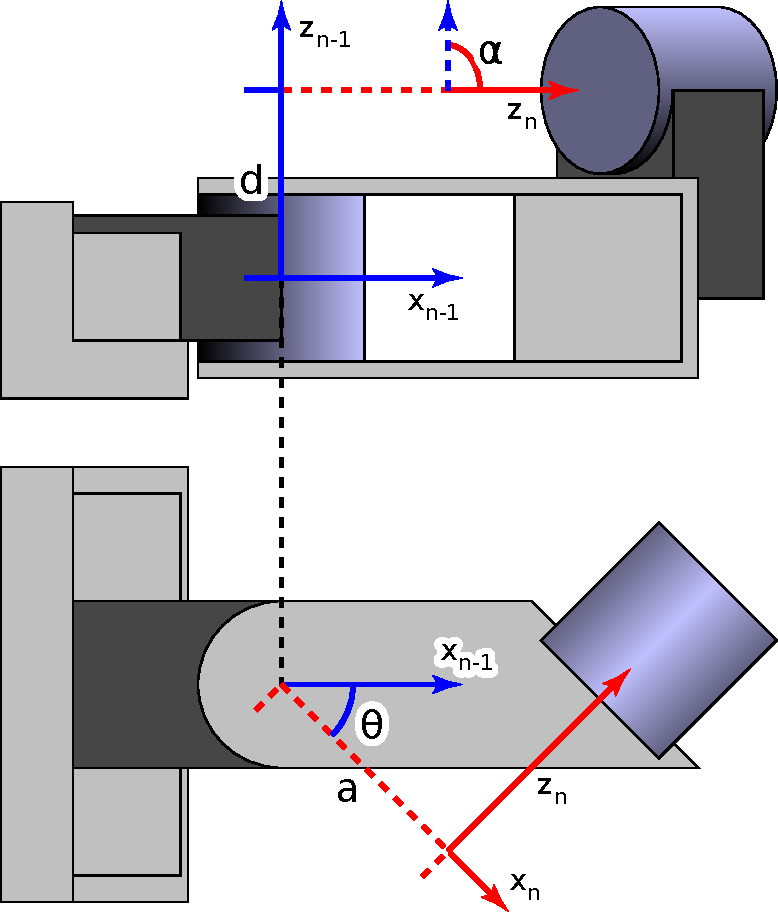
\includegraphics[height=.4\textheight]{Figures/Sample_Denavit-Hartenberg_Diagram.pdf}
 		\caption{Denavit-Hartenberg (DH) parameters: $a$, $\alpha$, $d$, and $\theta$~\cite{tekkotsu}}
 		\label{fig:DH}
	\end{center}
\end{figure}

Now, we can move from the base reference frame of some joint to the transformed reference frame of this joint using the transformation matrix $T_{DH}$, which consists of two translations and two rotations parametrized by the DH parameters of the joint:
\[T_{DH} = R_x(\alpha)T_x(a)R_z(\theta)T_z(d)\]
The analytical form of the resulting matrix from the above composition is the following:
\[
T_{DH} = 
\begin{bmatrix}
\cos\theta & -\sin\theta & 0 & a\\
\sin\theta\cos\alpha & \cos\theta\cos\alpha & -\sin\alpha & -d\sin\alpha\\
\sin\theta\cos\alpha & \cos\theta\sin\alpha & \cos\alpha & d\cos\alpha\\
0 & 0 & 0 & 1
\end{bmatrix}
\]
It is easy to see that the matrix above is an affine transformation matrix, because it is the product of affine transformation matrices.

\section{Mathematica}
Mathematica$^{\textrm{\copyright}}$ is a software tool for mathematical computations created by the Wolfram company (\url{www.wolfram.com}). This tool is widely-used, because, among other things, it can easily find solutions to differential equations and can perform symbolic computations. For the purposes of this thesis, we exploited its capability to perform large-scale symbolic computations with matrices and simplify symbolic expressions in reasonable time.

The following code excerpt is a small example of symbolic computation with Mathematica. We construct two matrices with cosines and sines containing two symbols, {\tt theta1} and {\tt theta2}. Next, we multiply those two matrices symbolically and finally we simplify the result:

\begin{small}
\begin{verbatim}
Matrix1 = {{Cos[theta1], -Sin[theta1]}, {Cos[theta1], -Cos[theta1]}};
Matrix2 = {{Cos[theta2], -Sin[theta2]}, {Cos[theta2], -Cos[theta2]}};
T = Matrix1.Matrix2;
Simplify[T];
MatrixForm[%]
\end{verbatim}
\end{small}

\noindent
The result of these symbolic computations is the following:
\begin{align*}
\text{Matrix1} &= \begin{bmatrix}
\cos\theta_1 & -\sin\theta_1\\
\cos\theta_1 & -\cos\theta_1
\end{bmatrix}\\
\text{Matrix2} &= \begin{bmatrix}
\cos\theta_2 & -\sin\theta_2\\
\cos\theta_2 & -\cos\theta_2
\end{bmatrix}\\
\text{T} &= \begin{bmatrix}
\cos\theta_1\cos\theta_2 - \cos\theta_2\sin\theta_1 &   \cos\theta_2 \sin\theta_1 - \cos\theta_1 \sin\theta_2\\
0 & \cos\theta_1 \cos\theta_2 - \cos\theta_1 \sin\theta_2
\end{bmatrix}\\
\text{T}_{\text{simplified}} &= \begin{bmatrix}
\cos\theta_2\left(\cos\theta_1 - \sin\theta_1\right) & \sin\left(\theta_1 - \theta_2\right)\\
 0 & \cos\theta_1 \left(\cos\theta_2 - \sin\theta_2\right)
\end{bmatrix}
\end{align*}
The example above is quite simple, but fully illustrates the symbolic capabilities of Mathematica and particularly the simplification step, which is very important for our work, given that we have to deal with much larger and more complex matrices.
 
\chapter{Problem statement}
\label{problem}

\section{The NAO Robot}
Aldebaran NAO is a humanoid robot. It is 58 cm tall and it has 5kg approximate mass. The version we are working on is the RoboCup version 3.3 with 21 DOF. It has 2 DOF on the head, 4 on each arm and 5 on each leg and 1 DOF that is common between the two legs. NAO has five kinematic chains and they are the following:
\begin{itemize}
\item Head chain: HeadYaw, HeadPitch.
\item Left Arm chain: LShoulderPitch, LShoulderRoll, LElbowYaw, LElbowRoll.
\item Right Hand chain: RShoulderPitch, RShoulderRoll, RElbowYaw, RElbowRoll.
\item Left Leg chain: LHipYawPitch, LHipRoll, LHipPitch, LKneePitch, LAnklePitch, LAnkleRoll.
\item Right Leg chain: RHipYawPitch, RHipRoll, RHipPitch, RKneePitch, RAnklePitch, RAnkleRoll.
\end{itemize}
The common joint is the HipYawPitch joint, so LHipYawPitch and RHipYawPitch are the same joint.

In the figure bellow we are presenting the academic edition of NAO. NAO RoboCup edition misses 4 DOF on the hand (LWristYaw, LHand, RWristYaw and RHand).
\begin{figure}[h]
	\begin{center}
		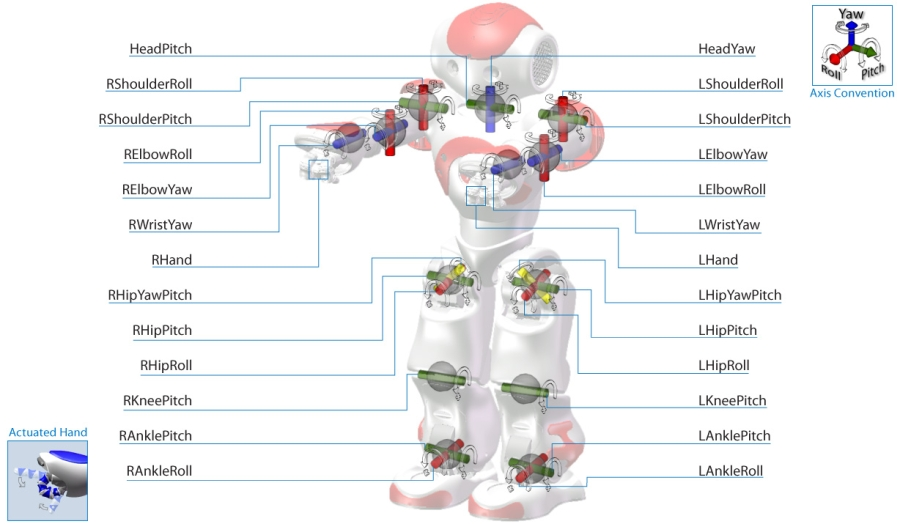
\includegraphics[height = 10cm]{Figures/nao-robot-dof.jpeg}
 		\caption{Aldebaran NAO V3.3 DOF of Academic Edition}
 		\label{fig:NAO}
	\end{center}
\end{figure}
\subsection{NAO Cartesian Restrictions}
In the figures and the tables bellow we will present the length of all the links of the robot (Table~\ref{fig:NAOlinks}) , the range that each joint is working in radians and in degrees (Figures~\ref{fig:hjoints},~\ref{fig:ajoints},~and~\ref{fig:ljoints}) and finally the masses of the NAO (Table~\ref{tab:Masses of NAO}). Each joint has its own mass and center of mass. The center of mass for each joint is represented by a point in the three-dimensional space of the joint. The robot theoretically is symmetric but we will see, in the joints ranges, that some left joints have different range than the right ones. The values are extracted from the user manual of the robot that Aldebaran provides.
The user manual has only masses for the right part of the robot but we assume that the robot is fully symmetrical on the masses.
Although some joints appear to be able to go to a position, the hardware controller of the robot will prohibit this movement because of the possible collisions with NAO shell.

\begin{figure}
\begin{tabular}{p{9cm}l|l|}
\multirow{14}{*}{
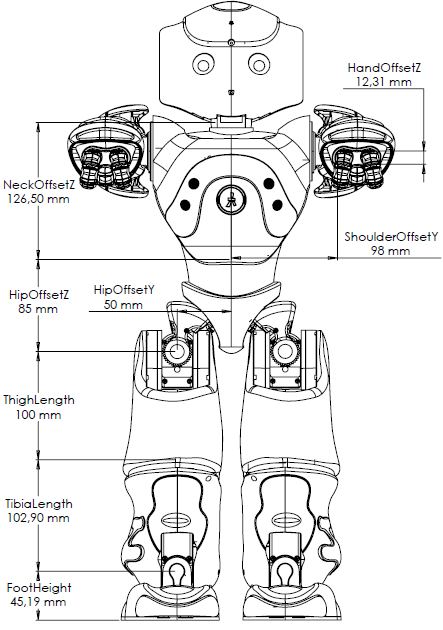
\includegraphics[height = 9cm]{Figures/naolinks_1.png}
}& \multicolumn{2}{c}{} \\
& \multicolumn{2}{c}{} \\
& \multicolumn{2}{c}{} \\
& \multicolumn{2}{c}{} \\
& \multicolumn{2}{c}{} \\
\cline{2-3}
& \multicolumn{1}{|l|}{\textbf{Name}} & \textbf{Size (mm)} \\ \cline{2-3}
& \multicolumn{1}{|l|}{NeckOffsetZ} & 126.50 \\ \cline{2-3}
& \multicolumn{1}{|l|}{ShoulderOffsetY} & 98.00 \\ \cline{2-3}
& \multicolumn{1}{|l|}{ElbowOffsetY} & 15.00 \\ \cline{2-3}
& \multicolumn{1}{|l|}{UpperArmLength} & 105.00 \\ \cline{2-3}
& \multicolumn{1}{|l|}{LowerArmLength} & 55.95 \\ \cline{2-3}
& \multicolumn{1}{|l|}{ShoulderOffsetZ} & 100.00 \\ \cline{2-3}
& \multicolumn{1}{|l|}{HandOffsetX} & 57.75 \\ \cline{2-3}
 & \multicolumn{1}{|l|}{HipOffsetZ} & 85.00 \\ \cline{2-3}
\multirow{10}{*}{
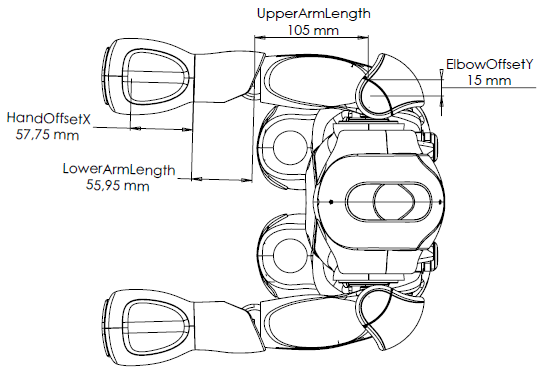
\includegraphics[height = 5cm]{Figures/naolinks_2.png}
}& \multicolumn{1}{|l|}{HipOffsetY} & 50.00 \\ \cline{2-3}
& \multicolumn{1}{|l|}{ThighLength} & 100.00 \\ \cline{2-3}
& \multicolumn{1}{|l|}{TibiaLength} & 102.90 \\ \cline{2-3}
& \multicolumn{1}{|l|}{FootHeight} & 45.19 \\ \cline{2-3}
& \multicolumn{1}{|l|}{HandOffsetZ} & 12.31 \\\cline{2-3}
& \multicolumn{2}{c}{} \\
& \multicolumn{2}{c}{} \\
& \multicolumn{2}{c}{} \\
& \multicolumn{2}{c}{} \\
& \multicolumn{2}{c}{} \\

\end{tabular}
\caption{NAO links sizes}
\label{fig:NAOlinks}
\end{figure}

\begin{figure}
\begin{tabular}{|p{5cm}|p{5cm}|p{5cm}|}
\multicolumn{3}{p{15cm}}{\centering 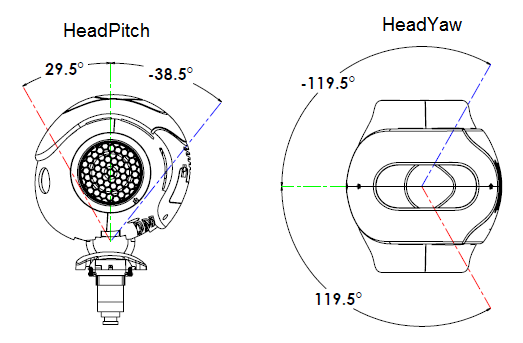
\includegraphics[height = 3.5cm]{Figures/headjoints.png}} \\ \hline
\textbf{Joint Name} & \textbf{Range in Degrees$^{\circ}$} & \textbf{Range in Radians} \\ \hline
HeadYaw & -119.5$^{\circ}$ to 119.5$^{\circ}$ & -2.0857 to 2.0857 \\ \hline
HeadPitch & -38.5$^{\circ}$ to 29.5$^{\circ}$ & -0.6720 to 0.5149 \\ \hline
\end{tabular}
\caption{Head joints range}
\label{fig:hjoints}
\end{figure}

\begin{figure}
\begin{tabular}{|p{5cm}|p{5cm}|p{5cm}|}
\multicolumn{3}{p{15cm}}{\centering 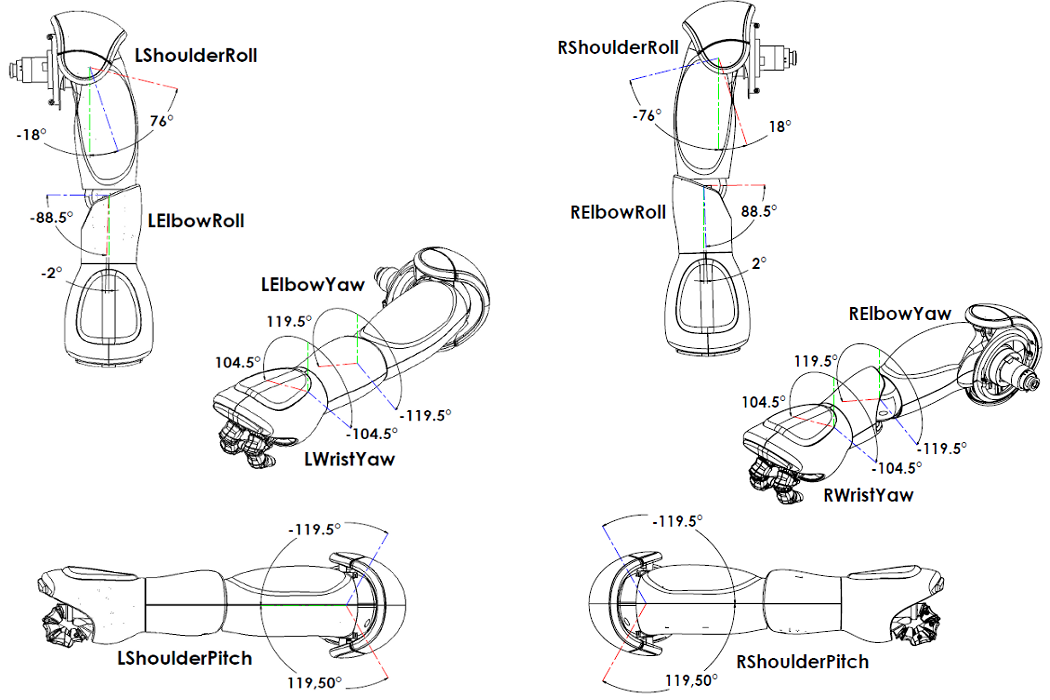
\includegraphics[height = 6.5cm]{Figures/armsjoints.png}} \\ \hline
\textbf{Joint Name} & \textbf{Range in Degrees$^{\circ}$} & \textbf{Range in Radians} \\ \hline
LShoulderPitch & -119.5$^{\circ}$ to 119.5$^{\circ}$ & -2.0857 to 2.0857 \\ \hline
LShoulderRoll & -18$^{\circ}$ to 76$^{\circ}$ & -0.3142 to 1.3265 \\ \hline
LElbowYaw & -119.5$^{\circ}$ to 119.5$^{\circ}$ & 1.5446 to 0.0349 \\ \hline
LElbowRoll & -88.5$^{\circ}$ to -2$^{\circ}$ & -0.6720 to 0.5149 \\ \hline
RShoulderPitch & -119.5$^{\circ}$ to 119.5$^{\circ}$ & -2.0857 to 2.0857 \\ \hline
RShoulderRoll & -38.5$^{\circ}$ to 29.5$^{\circ}$ & -1.3265 to 0.3142 \\ \hline
RElbowYaw & -119.5$^{\circ}$ to 119.5$^{\circ}$ & -2.0857 to 2.0857 \\ \hline
RElbowRoll & -38.5$^{\circ}$ to 29.5$^{\circ}$ & 0.0349 to 1.5446 \\ \hline
LWristYaw and RWristYaw & disabled & disabled \\ \hline
\end{tabular}
\caption{Arms joints range}
\label{fig:ajoints}
\end{figure}

\begin{figure}
\begin{tabular}{|p{5cm}|p{5cm}|p{5cm}|}
\multicolumn{3}{p{15cm}}{\centering 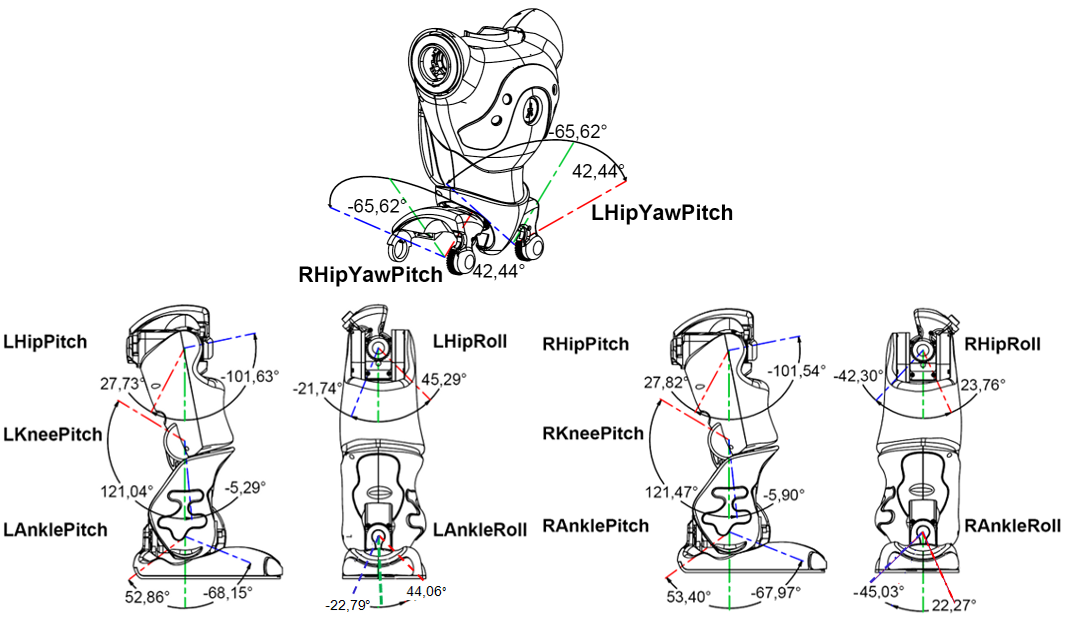
\includegraphics[width = 15cm]{Figures/legsjoints.png}} \\ \hline
\textbf{Joint Name} & \textbf{Range in Degrees$^{\circ}$} & \textbf{Range in Radians} \\ \hline
LHipYawPitch-RHipYawPitch & -65.62 to 42.44 & -1.145303 to 0.740810 \\ \hline
LHipRoll & -21.74$^{\circ}$ to 45.29$^{\circ}$ & -0.379472 to 0.790477 \\ \hline
LHipPitch & -101.63$^{\circ}$ to 27.73$^{\circ}$ & -1.773912 to 0.484090 \\ \hline
LKneePitch & -5.29$^{\circ}$ to 121.04$^{\circ}$ & -0.092346 to 2.112528 \\ \hline
LAnklePitch & -68.15$^{\circ}$ to 52.86$^{\circ}$ & -1.189516 to 0.922747 \\ \hline
LAnkleRoll & -22.79$^{\circ}$ to 44.06$^{\circ}$ & -0.397880 to 0.769001 \\ \hline
RHipRoll & -42.30$^{\circ}$ to 23.76$^{\circ}$ & -0.738321 to 0.414754 \\ \hline
RHipPitch & -101.54$^{\circ}$ to 27.82$^{\circ}$ & -1.772308 to 0.485624 \\ \hline
RKneePitch & -5.90$^{\circ}$ to 121.47$^{\circ}$ & -0.103083 to 2.120198 \\ \hline
RAnklePitch & -67.97$^{\circ}$ to 53.40$^{\circ}$ & -1.186448 to 0.932056 \\ \hline
RAnkleRoll & -45.03$^{\circ}$ to 22.27$^{\circ}$ & -0.785875 to 0.388676 \\ \hline
\end{tabular}
\caption{Legs joints range}
\label{fig:ljoints}
\end{figure}

\begin{table}[position specifier]
\caption{Masses of NAO}
\begin{tabular}{|l|r|r|r|r|}
\hline
\multicolumn{5}{|c|}{\textbf{Masses for NAO v3.3 robocup edition (H21)}} \\ \hline
\multicolumn{3}{|l|}{Total Mass For NAO H21} & \multicolumn{2}{|r|}{4.879 kg}\\ \hline
\textbf{Frame Name} & \textbf{Mass (Kg)} & \textbf{CoM$_{\text{x}}$ (mm)} & \textbf{CoM$_{\text{y}}$ (mm)} & \textbf{CoM$_{\text{z}}$ (mm)}\\ \hline
Torso & 1.03948 & -4.15 & 0.07 & 42.58 \\ \hline
HeadYaw & 0.05930 & -0.02 & 0.17 & 25.56 \\ \hline
HeadPitch & 0.52065 & 1.2 & -0.84 & 53.53 \\ \hline
RShoulderPitch & 0.06996 & -1.78 & 24.96 & 0.18 \\ \hline
RShoulderRoll & 0.12309 & 18.85 & -5.77 & 0.65 \\ \hline
RElbowYaw & 0.05971 & -25.6 & 0.01 & -0.19 \\ \hline
RElbowRoll & 0.185 & 65.36 & -0.34 & -0.02 \\ \hline
LShoulderPitch & 0.06996 & -1.78 & -24.96 & 0.18 \\ \hline
LShoulderRoll & 0.12309 & 18.85 & 5.77 & 0.65 \\ \hline
LElbowYaw & 0.05971 & -25.6 & -0.01 & -0.19 \\ \hline
LElbowRoll & 0.185 & 65.36 & 0.34 & -0.02 \\ \hline
RHipYawPitch & 0.07117 & -7.66 & 12 & 27.17 \\ \hline
RHipRoll & 0.1353 & -16.49 & -0.29 & -4.75 \\ \hline
RHipPitch & 0.39421 & 1.32 & -2.35 & -53.52 \\ \hline
RKneePitch & 0.29159 & 4.22 & -2.52 & -48.68 \\ \hline
RAnklePitch & 0.13892 & 1.42 & -0.28 & 6.38 \\ \hline
RAnkleRoll & 0.16175 & 25.4 & -3.32 & -32.41 \\ \hline
LHipYawPitch & 0.07117 & -7.66 & -12 & 27.17 \\ \hline
LHipRoll & 0.1353 & -16.49 & 0.29 & -4.75 \\ \hline
LHipPitch & 0.39421 & 1.32 & 2.35 & -53.52 \\ \hline
LKneePitch & 0.29159 & 4.22 & 2.52 & -48.68 \\ \hline
LAnklePitch & 0.13892 & 1.42 & 0.28 & 6.38 \\ \hline
LAnkleRoll & 0.16175 & 25.4 & 3.32 & -32.41 \\ \hline
\end{tabular}
\label{tab:Masses of NAO}
\end{table}

\newpage
\section{Kinematics for NAO}
Because NAO has a lot of DOF, it can do several complex moves. Some examples of those complex moves are walking, kicking a ball, standing up etc. NAO has five kinematic chains, three of them completely independent and two of them with one common joint. Kinematics is very useful for the programmers of NAO because they can create dynamic movements with the use of inverse kinematics or they can find the horizon of the camera on the head of the robot using forward kinematics.
\subsection{The Forward Kinematics problem for NAO}
Forward kinematics for NAO can been seen as five individual solutions. NAO has five chains and because we will not manipulate the joints, but we will only take the current state of each joint, we can assume that the five chains are completely independent. Then, we can find five forward kinematics solutions, one for each kinematic chain and we will be able to combine these solutions to find a solution for a bigger kinematic chain (e.g. the kinematic chain from the right foot to the head). The reason for dealing with this problem is twofold:firstly it is of great importance (concerning many applications, such as, finding its horizon, as well as placing it correctly).Besides this, as it will be described below, solution to the inverse kinematics problem would be intractable without solving the forward first.

\subsection{The Inverse Kinematics problem for NAO}
The inverse kinematics problem is a more complex problem and although we have the common joint between two kinematic chains, we are working with the assumption that we have five completely independent kinematic chains, so we will find five solutions for this problem. The reasons that led us to solve it are many. More specifically, we need to create dynamic kicks and an omni-directional walk. Both problems need a mechanism to move trajectories from the three-dimensional space to the joint space and the inverse kinematics can provide this mechanism.
\subsubsection*{Analytic versus Approximate solutions}
Inverse kinematics problem can be solved analytically or approximately. We have chosen to find the analytical solution rather than the approximate solution because the second one has some problems. We need real-time execution to the problem of inverse kinematics. The analytical solution is faster than the fastest approximate solution and for this reason it is a good choice for real-time execution. Second, there are various implementations of approximate solutions for the problem. Some of them are fast but it is very possible to run into a singularity. Other methods have a smaller probability to run into a singularity, but they are slower. On the other hand, the analytical solution doesn't have any singularity. However, inverse kinematics have an analytical solution only if the chain has five or less DOF. If the chain has 6 DOF, it can have analytical solution to the problem of the inverse kinematics only if three sequential joints have intersecting axes.
% ------------------------------------------------------------------------

%%% Local Variables:
%%% mode: latex
%%% TeX-master: "../thesis"
%%% End:

 \chapter{Related Work}
\label{related}

The problem of forward and inverse kinematics for the NAO robot is a familiar problem to all the teams participating in RoboCup SPL. The solution to forward kinematics is quite straightforward and most teams have implemented their own code for forward kinematics computations. There are only a few known solutions for the problem of inverse kinematics. We review existing related work in the next few sections. 

\section{Aldebaran Robotics}

\subsubsection*{Aldebaran Forward Kinematics Solution}
Aldebaran Robotics provides a forward kinematics mechanism integrated within the proprietary NaoQi middleware for the NAO robot. However, this mechanism does not accept any input and provides a solution only for the current joint configuration of the robot. As a result, it is impossible to run Aldebaran's forward kinematics for a specific set of joint values, for example the joint values recorded when a specific picture was acquired from the camera. The ability to provide any set of joints is important, not only for finding the position of the camera in the three-dimensional at specific times, but also for verifying candidate solutions returned by inverse kinematics. On the other hand, Aldebaran provides the DH parameters for all the joints of the NAO robot and that was very useful.

\subsubsection*{Aldebaran Inverse Kinematics Solution}
Aldebaran Robotics provides an inverse kinematics mechanism integrated within the proprietary NaoQi middleware for the NAO robot. These functions in the API of the robot can move the end effector of a kinematic chain to a given point in the three-dimensional space. The method used to provide the solution is based on the Jacobian iterative approximation method. Furthermore, the omni-directional walk engine provided by Aldebaran Robotics uses this approach to follow planned foot trajectories. Although the resulting solutions are in most cases accurate, the method can easily fall into singularities; if that happens, the robot gets stuck in a specific configuration. Singularities present a serious problem with possible catastrophic consequences for the robot. 

\section{B-Human Inverse Kinematics Solution}
B-Human is the RoboCup SPL team of the University of Bremen in Germany. Each year they publish a code release, which includes the full code they used in the last RoboCup and a documentation for this code. In their recent code release~\cite{bhuman} they include an inverse kinematics solution for the legs of NAO, albeit with under certain simplification assumptions and approximations. The solution provided always makes the foot parallel to the plane defined by the $z$-axis and the $x$-axis of the torso. If the target point violates this assumption, the solution will reach the target position, but will ignore the target orientation, and therefore it will only be an approximate solution. 

\section{QIAU Inverse Kinematics Solution}
MRL is the RoboCup SPL team of the Qazvin Islamic Azad University (QIAU) in Tehran, Iran. They have published~\cite{iran} an analytical solution for the problem of inverse kinematics for the legs. We have tried to implement their solution, but unfortunately we were not able to reproduce their results.
 \chapter{NAO Kinematics: The Solution}
\label{approach}

As mentioned in Chapter~\ref{related}, the existing approaches to kinematics for the NAO robot are not completely suitable for our needs. We seek to find a solution to the forward kinematics problem for any set of joint values as input and not only for the current joint values. In addition, we seek to find a real-time analytical solution for the problem of inverse kinematics without any approximations. In the sections below, we describe our solutions to both of these problems.


\section{Forward Kinematics for the NAO Robot}


Aldebaran Robotics provides the DH parameters for each kinematic chain of the robot in the documentation~\cite{AldebaranNaoDoc}. However, our experimentation with the provided values revealed that the given parameters for the arm chains are incorrect. Therefore, we found our own parameters for the arms and we used the provided parameters for the legs and the head.


\subsubsection*{NAO Zero Position}
We must define the base frame of the robot and the zero position of the joints before we proceed. The base frame is taken to be the torso frame; Figure~\ref{fig:torso} shows the axes of this frame. The same figure shows also the zero position of all the joints of the robot, which is the one provided by Aldebaran Robotics. As we can see, in this position the ShoulderRoll joints are not really roll joints, but are yaw joints, so we can understand that the names of the joints do not necessarily describe the actual movement of the joint in the base frame given the zero position.

\begin{figure}[h]
\begin{center}
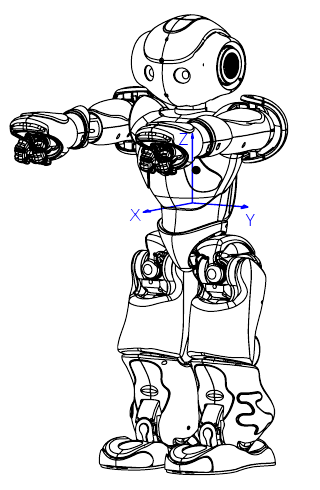
\includegraphics[height = 10cm]{Figures/torso_frame.png}
\caption{Base (torso) frame and zero position of the joints}
\label{fig:torso}
\end{center}
\end{figure}


\subsubsection*{Notation}
We provide a brief description of the symbols we use in our math calculations. All matrices used are affine transformation matrices of three types: $T$ is a transformation matrix, $R_x, R_y, R_z$ are basic rotations matrices, and $A$ is a translation matrix. The subscript of a symbol refers to the start frame and the superscript refers to the destination frame. The torso is the point where all the kinematic chains begin and is located at the center of the NAO body. ``Base'' is the start frame of the chain (the torso frame), while ``End'' is the end effector of the chain. The numbers appearing as subscripts or superscripts refer to the joints in the current kinematic chain, numbered consistently with the ordering given in the tables of Chapter~\ref{problem}. Also, we denote the initialization of a translation matrix as $A(d_x,d_y,d_z)$ and of rotation matrices as $R_x(\theta_x)$, $R_y(\theta_y)$, or $R_z(\theta_z)$.

We present the DH parameters of each kinematic chain in a separate table and, besides the DH parameters, we provide the translations from the ``Base'' to the first joint and from the last joint to the ``End''. Finally, we provide some necessary rotations to adjust the frame of the last joint to the frame of the end effector (``End'').


\subsubsection*{Forward Kinematics Equations}
Forward kinematics for each chain of the NAO robot is a transformation that maps a point from the frame of the last joint to the base frame. In our case, the end effector is the point of interest. Forward kinematics are defined in terms of transformation, rotation, and translation matrices, and the final result is a single transformation matrix that maps points from one frame to another. 

\subsubsection*{Extracting the Point in the Three-Dimensional Space}
The result of forward kinematics is an affine transformation matrix $T$ with the $X$ block being a rotation matrix and the $Y$ block being a translation vector. We need to extract the $(p_x, p_y, p_z)$ position and the $(a_x,a_y,a_z)$ orientations of the final point. The position $(p_x, p_y, p_z)$ can be simply read off the translation part of the transformation matrix:
\begin{align*}
p_x &= T_{(1,4)}\\
p_y &= T_{(2,4)}\\
p_z &= T_{(3,4)}
\end{align*}
The rotation of the final transformation table is a $R_zR_yR_x$ rotation table, whose analytical form is shown in Section~\ref{sec:affine}. Now it's easy to extract the orientation $(a_x,a_y,a_z)$:
\begin{align*}
a_x &= \arctan\!2 \left(T_{(3,2)},T_{(3,3)}\right)\\
a_y &= \arctan\!2 \left(-T_{(3,1)},\sqrt{{T_{(3,2)}}^2 + {T_{(3,3)}}^2}\right)\\
a_z &= \arctan\!2 \left(T_{(2,1)},T_{(1,1)}\right)
\end{align*}

\subsection{Forward Kinematics for the Head}
The head is the simplest kinematic chain of the NAO robot, but it has two useful end effectors, namely the top and the bottom cameras. Table~\ref{tab:DHhead} shows the DH parameters for the head chain. Now, we can combine these matrices to find the point of the end effector in the frame space of the torso:
\[
T^\text{End}_\text{Base} = A^0_\text{Base}T^1_0T^2_1R_x(\tfrac{\pi}{2})R_y(\tfrac{\pi}{2})A^\text{End}_{2}
\]
$T^1_0$ and $T^2_1$ are the DH transformation matrices of the corresponding joints (HeadYaw, HeadPitch). $A^\text{End}_{2}$ is one of the two translation matrices given in Table~\ref{tab:DHhead} for the two end effectors (top and bottom camera). The point of the end effector in the three-dimensional space of the torso can be extracted from $T^\text{End}_\text{Base}$.


\begin{table}[t!]
\centering
\caption{DH parameters for the Head chain}
\begin{tabular}{|l|>{\centering\arraybackslash}m{2.55cm}|>{\centering\arraybackslash}m{2.55cm}|>{\centering\arraybackslash}m{2.55cm}|>{\centering\arraybackslash}m{2.55cm}|}
\hline
\textbf{Frame (Joint)} & $\mathbf{a}$ & $\boldsymbol{\alpha}$ & $\mathbf{d}$ & $\boldsymbol{\theta}$\\ \hline
Base & \multicolumn{4}{c|}{$A(0,0,\text{\footnotesize{NeckOffsetZ}})$} \\ \hline
HeadYaw & $0$ & $0$ & $0$ & $\theta_1$ \\ \hline
HeadPitch & $0$ & $-\frac{\pi}{2}$ & $0$ & $\theta_2 - \frac{\pi}{2}$ \\ \hline
Rotation & \multicolumn{4}{c|}{$R_x(\frac{\pi}{2})R_y(\frac{\pi}{2})$} \\ \hline
Top Camera & \multicolumn{4}{c|}{$A(\text{\footnotesize{topCameraX}},0,\text{\footnotesize{topCameraZ}})$} \\ \hline
Bottom Camera & \multicolumn{4}{c|}{$A(\text{\footnotesize{bottomCameraX}},0,\text{\footnotesize{bottomCameraZ}})$} \\ \hline
\multicolumn{5}{|c|}{\footnotesize{topCameraX=53.9mm, topCameraZ=67.9mm, bottomCameraX=48.8mm, bottomCameraZ=23.8mm}} \\ \hline
\end{tabular}
\label{tab:DHhead}
\end{table}

\subsection{Forward Kinematics for the Left Arm}

The kinematic chain for the left arm consists of four joints. So, we need to find four sets of DH parameters, one for each joint. First, we must move from the torso to the base of the joint and we can do that with a simple translation along the $y$-axis and the $z$-axis. After that, we must align the coordinate frame with the rotation axis of the first joint (LShoulderPitch). So, we rotate about the $x$-axis of the coordinate frame by $-\frac{\pi}{2}$, thus the $\alpha$ parameter for LShoulderPitch is $-\frac{\pi}{2}$, while $d$, $a$ are $0$. Now, we must rotate the coordinate frame again to become aligned with the rotation axis of the second joint (LShoulderRoll). So, we rotate about the $x$-axis by $\frac{\pi}{2}$, thus the $\alpha$ parameter for LShoulderRoll is $\frac{\pi}{2}$, while $d$, $a$ are $0$. Next, we need to align the coordinate frame with the rotation axis of the third joint (LElbowYaw). To do so, we must rotate about the $y$-axis. The DH parameters do not directly encode a rotation about the $y$-axis, so we must first rotate about the $z$-axis and then about the $x$-axis to effectively realize a rotation about the $y$-axis. Thus, we subtract $-\frac{\pi}{2}$ from the angle $\theta_2$ of the previous joint (to rotate about the $z$-axis) and then rotate about the $x$-axis by $-\frac{\pi}{2}$ (the $\alpha$ parameter of LElbowYaw). Then, we move along the $z$-axis to reach the position of the LElbowYaw joint, so its $d$ parameter is set to UpperArmLength and $a$ is $0$. Finally, for the fourth joint (LElbowRoll) we rotate about the $x$-axis by $\frac{\pi}{2}$, thus the $\alpha$ parameter for LElbowRoll is $\frac{\pi}{2}$, while $d$, $a$ are $0$. At the end, we only need a simple rotation to fix the orientation of our coordinate frame and a simple translation to reach the end effector.



\begin{table}[t!]
\centering
\caption{DH parameters for the Left Arm chain}
\begin{tabular}{|l|>{\centering\arraybackslash}m{2.55cm}|>{\centering\arraybackslash}m{2.55cm}|>{\centering\arraybackslash}m{2.55cm}|>{\centering\arraybackslash}m{2.55cm}|}
\hline
\textbf{Frame (Joint)} & $\mathbf{a}$ & $\boldsymbol{\alpha}$ & $\mathbf{d}$ & $\boldsymbol{\theta}$\\ \hline
Base & \multicolumn{4}{c|}{$A(0,\text{\footnotesize{ShoulderOffsetY+ElbowOffsetY}},\text{\footnotesize{ShoulderOffsetZ}})$} \\ \hline
LShoulderPitch & $0$ & $-\frac{\pi}{2}$ & $0$ & $\theta_1$ \\ \hline
LShoulderRoll & $0$ & $\frac{\pi}{2}$ & $0$ & $\theta_2 - \frac{\pi}{2}$ \\ \hline
LElbowYaw & $0$ & $-\frac{\pi}{2}$ & \footnotesize{UpperArmLength} & $\theta_3$ \\ \hline
LElbowRoll & $0$ & $\frac{\pi}{2}$ & $0$ & $\theta_4$ \\ \hline
Rotation & \multicolumn{4}{c|}{$R_z(\frac{\pi}{2})$} \\ \hline
End effector & \multicolumn{4}{c|}{$A(\text{\footnotesize{HandOffsetX+LowerArmLength}},0,0)$} \\ \hline
\end{tabular}
\label{tab:DHlarm}
\end{table}

Table~\ref{tab:DHlarm} shows the DH parameters for all the joints of the left arm chain along with the necessary translations and rotations.
Now, we can easily calculate the final transformation matrix:
\[
T^\text{End}_\text{Base} = A^0_\text{Base}T^1_0T^2_1T^3_2T^4_3R_z(\tfrac{\pi}{2})A^\text{End}_{4}
\]

\subsection{Forward Kinematics for the Right Arm}
The kinematic chain of the right arm is fully symmetric with the left arm chain relatively to the plane defined by the $x$-axis and the $z$-axis. So, the differences between the two chains are only in the distances along the $y$-axis and in the joints that rotate about the $y$-axis. Also, in this chain we must add one extra rotation matrix after the final translation, because the $z$-axis is inverted. All the DH parameters for this chain can be seen in Table~\ref{tab:DHrarm} and the final transformation matrix is:
\[
T^\text{End}_\text{Base} = A^0_\text{Base}T^1_0T^2_1T^3_2T^4_3R_z(\tfrac{\pi}{2})A^\text{End}_{4}R_z(-\pi)
\]

\begin{table}[!t]
\centering
\caption{DH parameters for Right Arm chain}
\begin{tabular}{|l|>{\centering\arraybackslash}m{2.55cm}|>{\centering\arraybackslash}m{2.55cm}|>{\centering\arraybackslash}m{2.85cm}|>{\centering\arraybackslash}m{2.55cm}|}
\hline
\textbf{Frame (Joint)} & $\mathbf{a}$ & $\boldsymbol{\alpha}$ & $\mathbf{d}$ & $\boldsymbol{\theta}$\\ \hline
Base & \multicolumn{4}{c|}{$A(0,\text{\footnotesize{$-$ShoulderOffsetY $-$ ElbowOffsetY}},\text{\footnotesize{ShoulderOffsetZ}})$} \\ \hline
RShoulderPitch & $0$ & $-\frac{\pi}{2}$ & $0$ & $\theta_1$ \\ \hline
RShoulderRoll & $0$ & $\frac{\pi}{2}$ & $0$ & $\theta_2 + \frac{\pi}{2}$ \\ \hline
RElbowYaw & $0$ & $-\frac{\pi}{2}$ & \footnotesize{$-$UpperArmLength} & $\theta_3$ \\ \hline
RElbowRoll & $0$ & $\frac{\pi}{2}$ & $0$ & $\theta_4$ \\ \hline
Rotation & \multicolumn{4}{c|}{$R_z(\frac{\pi}{2})$} \\ \hline
End effector & \multicolumn{4}{c|}{$A(\text{\footnotesize{$-$HandOffsetX $-$ LowerArmLength}},0,0)$} \\ \hline
Rotation Fix & \multicolumn{4}{c|}{$R_z(-\pi)$} \\ \hline
\end{tabular}
\label{tab:DHrarm}
\end{table}



\subsection{Forward Kinematics for the Left Leg}
The kinematic chain for the left leg has six joints and it is the longest chain on the NAO robot. The DH parameters for these joints are interesting, because of the ``weird'' orientation of the HipYawPitch joint. Table~\ref{tab:DHlleg} shows the DH parameters for the entire kinematic chain of the left leg and the final transformation matrix is:
\[
T^\text{End}_\text{Base} = A^0_\text{Base}T^1_0T^2_1T^3_2T^4_3T^5_4T^6_5R_z(\pi)R_y(-\tfrac{\pi}{2})A^\text{End}_{6}
\]

\begin{table}[!t]
\centering
\caption{DH parameters for Left Leg chain}
\begin{tabular}{|l|>{\centering\arraybackslash}m{2.55cm}|>{\centering\arraybackslash}m{2.55cm}|>{\centering\arraybackslash}m{2.55cm}|>{\centering\arraybackslash}m{2.55cm}|}
\hline
\textbf{Frame (Joint)} & $\mathbf{a}$ & $\boldsymbol{\alpha}$ & $\mathbf{d}$ & $\boldsymbol{\theta}$\\ \hline
Base & \multicolumn{4}{c|}{$A(0,\text{\footnotesize{HipOffsetY}},\text{\footnotesize{$-$HipOffsetZ}})$} \\ \hline
LHipYawPitch & $0$ & $-\frac{3\pi}{4}$ & $0$ & $\theta_1 - \frac{\pi}{2}$ \\ \hline
LHipRoll & $0$ & $-\frac{\pi}{2}$ & $0$ & $\theta_2 + \frac{\pi}{4}$ \\ \hline
LHipPitch & $0$ & $\frac{\pi}{2}$ & $0$ & $\theta_3$ \\ \hline
LKneePitch & \footnotesize{$-$ThighLength} & $0$ & $0$ & $\theta_4$ \\ \hline
LAnklePitch & \footnotesize{$-$TibiaLength} & $0$ & $0$ & $\theta_5$ \\ \hline
LAnkleRoll & $0$ & $-\frac{\pi}{2}$ & $0$ & $\theta_6$ \\ \hline
Rotation & \multicolumn{4}{c|}{$R_z(\pi)R_y(-\tfrac{\pi}{2})$} \\ \hline
End effector & \multicolumn{4}{c|}{$A(0,0,\text{\footnotesize{$-$FootHeight}})$} \\ \hline
\end{tabular}
\label{tab:DHlleg}
\end{table}



\subsection{Forward Kinematics for the Right Leg}
Similarly to the arms, the kinematic chains for the legs are fully symmetric relatively to the plane defined by the $x$-axis and the $z$-axis. So, the differences between the two chains is only in the distances along the $y$-axis and in the joints that rotate about the $y$-axis. Table~\ref{tab:DHrleg} shows all the DH parameters for the right leg chain and the final transformation matrix is: 
\[
T^\text{End}_\text{Base} = A^0_\text{Base}T^1_0T^2_1T^3_2T^4_3T^5_4T^6_5R_z(\pi)R_y(-\tfrac{\pi}{2})A^\text{End}_{6}
\]

\begin{table}[!t]
\centering
\caption{DH parameters for Right Leg chain}
\begin{tabular}{|l|>{\centering\arraybackslash}m{2.55cm}|>{\centering\arraybackslash}m{2.55cm}|>{\centering\arraybackslash}m{2.55cm}|>{\centering\arraybackslash}m{2.55cm}|}
\hline
\textbf{Frame (Joint)} & $\mathbf{a}$ & $\boldsymbol{\alpha}$ & $\mathbf{d}$ & $\boldsymbol{\theta}$\\ \hline
Base & \multicolumn{4}{c|}{$A(0,\text{\footnotesize{$-$HipOffsetY}},\text{\footnotesize{$-$HipOffsetZ}})$} \\ \hline
RHipYawPitch & $0$ & $-\frac{\pi}{4}$ & $0$ & $\theta_1 - \frac{\pi}{2}$ \\ \hline
RHipRoll & $0$ & $-\frac{\pi}{2}$ & $0$ & $\theta_2 - \frac{\pi}{4}$ \\ \hline
RHipPitch & $0$ & $\frac{\pi}{2}$ & $0$ & $\theta_3$ \\ \hline
RKneePitch & \footnotesize{$-$ThighLength} & $0$ & $0$ & $\theta_4$ \\ \hline
RAnklePitch & \footnotesize{$-$TibiaLength} & $0$ & $0$ & $\theta_5$ \\ \hline
RAnkleRoll & $0$ & $-\frac{\pi}{2}$ & $0$ & $\theta_6$ \\ \hline
Rotation & \multicolumn{4}{c|}{$R_z(\pi)R_y(-\tfrac{\pi}{2})$} \\ \hline
End effector & \multicolumn{4}{c|}{$A(0,0,\text{\footnotesize{$-$FootHeight}})$} \\ \hline
\end{tabular}
\label{tab:DHrleg}
\end{table}


\subsection{Forward Kinematics for Combined Chains}
The forward kinematics transformations presented above assume the torso frame as the base frame. In practice, a NAO user may be interested in finding the point of the torso relatively to one of the feet. Note that this is the forward kinematics problem for the reverse chain. Given that the forward kinematics transformation matrices are affine transformation matrices, we can obtain the solution for this reverse problem by simply inverting the corresponding transformation matrix. 
For example, inverting the transformation matrix for the left leg chain yields a transformation matrix for the point of the torso in the frame of the left foot: 
\[
T^\text{Torso}_\text{LFoot} = {\left(T^\text{LFoot}_\text{Torso}\right)}^{-1}
\]
This solution reversion property of the forward kinematics allows the combination of multiple chains to obtain the point of the end effector of one chain in the frame of the end effector of the other chain through their common point (torso). 

For example, it is possible to find the point of the head relatively to the left foot. The kinematic chains for the head and for the left leg are relative to the torso frame. So, by inverting the transformation matrix of the left leg chain, we locate the torso relatively to the left foot frame. Then, we just multiply with the transformation matrix of the head chain and obtain a new transformation matrix that describes the point of the head relatively to the left foot frame.
\[
T^\text{Head}_\text{LFoot} = {\left(T^\text{LFoot}_\text{Torso}\right)}^{-1}T^\text{Head}_\text{Torso}
\]
This property is extremely useful, because we can describe any end effector relatively to the frame of any other end effector. For example, with this, we can find the exact height of the camera from the ground.

\subsection{Calculation of the Center Of Mass}
The Center of Mass (CoM) of a body in the three-dimensional space is a position, which corresponds to the weighted average location of all the mass in the body. From a physics point of view, the body (even if oddly-shaped) could be represented by a point mass located at the CoM. In humanoid robots, knowledge of the CoM is important to maintain balance. It is easy to see that the CoM changes, as the joint values change and the kinematic chains move in the three-dimensional space. 

The NAO robot consists of a group of connected parts (joints and the corresponding links). Each part has its own known mass and its own (local) CoM at a known static position. For any given configuration of the robot, forward kinematics can be applied to locate each of these parts in the three-dimensional space of the torso frame and from there calculate the exact position of the robot CoM relatively to the torso frame. 

Aldebaran Robotics provides the information needed for CoM calculations, in particular the mass of the whole robot and the masses of all parts of the robot. The mass of each distinct part is referenced by the corresponding joint of that part and its own local CoM is given relatively to its own joint frame.

The CoM of the entire robot is calculated relatively to the torso frame and the calculation order is simple. We first construct smaller kinematic chains, one for each of the 21 joints. Each of these smaller kinematic chains terminates at the corresponding joint and the position of the local CoM is set to be the end effector. We compute the forward kinematics for each of these 21 chains. Then, we extract the translation block of each transformation matrix and we multiply it with the mass of the corresponding part/joint. In total, we have 21 chains plus the torso chain (a zero-length chain). Finally, we add all the individual weighted translation matrices and the result is divided by the total mass of the robot. The outcome of this calculation is the position of the CoM relatively to the torso frame.











\section{Inverse Kinematics for NAO}


Forward kinematics can find the point of an end effector, relatively to the start frame, given the values of the joints. Now, we turn our attention to the inverse problem: find a set of values for the joints that drive a given end effector to a desired point relatively to the torso frame. The inverse kinematics presented below solve the problem for the five kinematic chains that start at the robot torso.

A point of the end effector in the three-dimensional space consists of a position $(p_x,p_y,p_z)$ and an orientation $(a_x,a_y,a_z)$. As mentioned above, the outcome of forward kinematics is an affine transformation matrix, which includes a rotation block and a translation block. The rotation block $R$ takes the form $R_zR_yR_x$. Thus, we can construct the complete transformation matrix $T$ from the base frame to the point of the end effector mentioned above:
\[
\begin{small}
T = 
\begin{bmatrix}
\cos a_y\cos a_z & -\cos a_x\sin a_z + \sin a_x\sin a_y\cos a_z & \sin a_x\sin a_z + \cos a_x\sin a_y\cos a_z & p_x\\
\cos a_y\sin a_z & \cos a_x\cos a_z + \sin a_x\sin a_y\sin a_z & -\sin a_x\cos a_z + \cos a_x\sin a_y\sin a_z & p_y\\
-\sin a_y & \sin a_x\cos a_y & \cos a_x\cos a_y & p_z\\
0 & 0 & 0 & 1
\end{bmatrix}
\end{small}
\]
Given $T$, our goal now is to find a set of joint values that leads to the same transformation through the kinematic chain. As mentioned before, the problem of inverse kinematics cannot be solved without the solution of forward kinematics. This is true, because the equations we must solve to find the values of the joints are formed by writing down the forward kinematics transformation matrix symbolically with the $\theta_i$'s of the DH parameters appearing as symbols in the matrix. This symbolic matrix is set to be equal to $T$ to yield twelve non-linear equations with the values $\theta_i$ of the $n$ joints of the chain as unknowns. In fact, we will have a total of $2n$ unknowns, because all the $\theta_i$'s appear inside a sine or a cosine, therefore for each joint $i$ there are two dependent unknowns in the system, $\sin\theta_i$ and $\cos\theta_i$.

As we shall see below, we obtain some of the solutions using $\arccos$ and $\arcsin$. The problem is that $\arcsin$ returns an angle in $\left[-\tfrac{\pi}{2},+\tfrac{\pi}{2}\right]$ and $\arccos$ returns an angle in $\left[0,\pi\right]$, even though the possible values of a joint can be in the range $\left[-\pi,+\pi\right]$. Thus, if $\theta^*_i$ is a value returned by $\arcsin$ or $\arccos$ as a solution, there is one additional symmetric solution, $\pi - \theta^*_i$ for $\arcsin$ and $-\theta^*_i$ for $\arccos$. Due to these symmetries, the equations lead to a small number of distinct candidate solutions, some of which may be infeasible or invalid because of the constrained range of each joint. To determine a valid and correct solution, we simply run each one of these solutions through the forward kinematics to verify that indeed the end effector of the chain reaches the desired position and orientation. Invalid solutions are discarded and only correct ones are kept. 


\subsection{Inverse Kinematics for the Head}
The head chain consists of only two joints, therefore we can work either with the position $(p_x,p_y,p_z)$ or with the orientation $(a_x,a_y,a_z)$ of the target point to obtain a solution. In the latter case, we can achieve the desired target orientation simply by setting the HeadYaw and HeadPitch joints to $a_z$ and $a_y$ respectively. In the former case, we first construct the symbolic matrix from forward kinematics along the head chain:
\[
T = 
\begin{bmatrix}
-\cos\theta_1\sin\widehat{\theta}_2 & -\sin\theta_1 & \cos\theta_1\cos\widehat{\theta}_2 &  l_2\cos\theta_1\cos\widehat{\theta}_2 - l_1\cos\theta_1\sin\widehat{\theta}_2\\
-\sin\theta_1\sin\widehat{\theta}_2 & \cos\theta_1 & \cos\widehat{\theta}_2\sin\theta_1 & l_2\cos\widehat{\theta}_2\sin\theta_1 - l_1\sin\theta_1\sin\widehat{\theta}_2\\
-\cos\widehat{\theta}_2 & 0 & -\sin\widehat{\theta}_2 & l_3 - l_2\sin\widehat{\theta}_2 - l_1\cos\widehat{\theta}_2\\
0 & 0 & 0 & 1
\end{bmatrix}
\]
where $\widehat{\theta}_2$ is the DH parameter $\theta$ for the second joint, $l_1 =$ cameraX, $l_2 =$ cameraZ, and $l_3 =$ NeckOffsetZ.
Since we only know the position $(p_x,p_y,p_z)$, we cannot reconstruct the rotation block of the matrix, so we focus on the translation block. From the symbolic matrix, we have: 
\[
T_{(3,4)} = l_3 - l_2\sin\widehat{\theta}_2 - l_1\cos\widehat{\theta}_2 = p_z
\]
We know from trigonometry that: 
\[
a\sin\theta + b\cos\theta = \sqrt{a^2+b^2}\sin\left(\theta + \psi\right)
\]
\[
\psi=\arctan\left(\frac{b}{a}\right) + \left\{ 
  \begin{array}{l l}
    0 & \quad \text{if }a\geq0\\
    \pi & \quad \text{if }a<0\\
  \end{array} \right.
\]
Given that $l_2>0$, we can now calculate $\widehat{\theta}_2$ as follows:
\[
\widehat{\theta}_2 = \arcsin\left(\cfrac{-p_z+l_3}{\sqrt{{l_1}^2+{l_2}^2}}\right) - \arctan\left(\frac{l_1}{l_2}\right)
\]
Now the final joint value $\theta_2$ is $\theta_2 = \widehat{\theta}_2 + \frac{\pi}{2}$.  From now on, we substitute $\theta_2 - \frac{\pi}{2}$ in $\widehat{\theta}_2$. Now, we can easily extract $\theta_1$ from $T_{(1,4)}$:
\[
\theta_1 = \arccos\left(\cfrac{p_x}{l_2\cos\left(\theta_2 - \frac{\pi}{2}\right) - l_1\sin\left(\theta_2 - \frac{\pi}{2}\right) } \right)
\]
So, the final inverse kinematics equations for the head chain are:
\begin{align*}
\theta_2 &= \arcsin\left(\cfrac{- p_z + l_3}{ \sqrt{{l_1}^2+{l_2}^2} }\right) - \arctan\left(\frac{l_1}{l_2}\right) + \frac{\pi}{2}\\
\theta_2 &= \pi - \arcsin\left(\cfrac{- p_z + l_3}{ \sqrt{{l_1}^2+{l_2}^2} }\right) - \arctan\left(\frac{l_1}{l_2}\right) + \frac{\pi}{2}\\
\theta_1 &= \pm\arccos\left(\cfrac{p_x}{l_2\cos\left(\theta_2 - \frac{\pi}{2}\right) - l_1\sin\left(\theta_2 - \frac{\pi}{2}\right) } \right)
\end{align*}
provided a target position $(p_x,p_y,p_z)$ or 
\begin{align*}
\theta_1 &= a_z\\
\theta_2 &= a_y
\end{align*}
provided a target orientation $(a_x,a_y,a_z)$.

\subsection{Inverse Kinematics for the Left Arm}
The left arm chain is far more complicated than the head chain. First, we construct the symbolic transformation matrix for the left arm chain:
\begin{align*}
T &= \begin{bmatrix}
r_{11} & r_{12} & r_{13} & r_{14}\\
r_{21} & r_{22} & r_{23} & r_{24}\\
r_{31} & r_{32} & r_{33} & r_{34}\\
0 & 0 & 0 & 1
\end{bmatrix}\\
r_{11} &= \sin\theta_4\left(\sin\theta_1\sin\theta_3 - \cos\theta_1\cos\widehat{\theta}_2\cos\theta_3\right) - \cos\theta_1\cos\theta_4\sin\widehat{\theta}_2\\
r_{12} &= \cos\theta_4\left(\sin\theta_1\sin\theta_3 - \cos\theta_1\cos\widehat{\theta}_2\cos\theta_3\right) + \cos\theta_1\sin\widehat{\theta}_2\sin\theta_4\\
r_{13} &= \cos\theta_3\sin\theta_1 + \cos\theta_1\cos\widehat{\theta}_2\sin\theta_3\\
r_{14} &= l_4\left(\sin\theta_4\left(\sin\theta_1\sin\theta_3 - \cos\theta_1\cos\widehat{\theta}_2\cos\theta_3\right) - \cos\theta_1\cos\theta_4\sin\widehat{\theta}_2\right) - l_3\cos\theta_1\sin\widehat{\theta}_2\\
r_{21} &= \cos\widehat{\theta}_2\cos\theta_4 - \cos\theta_3\sin\widehat{\theta}_2\sin\theta_4\\
r_{22} &= \cos\widehat{\theta}_2\sin\theta_4 - \cos\theta_3\cos\theta_4\sin\widehat{\theta}_2\\
r_{23} &= \sin\widehat{\theta}_2\sin\theta_3\\
r_{24} &= l_1 + l_3\cos\widehat{\theta}_2 + l_4\left(\cos\widehat{\theta}_2\cos\theta_4 - \cos\theta_3\sin\widehat{\theta}_2\sin\theta_4\right)\\
r_{31} &= \sin\theta_4\left(\cos\theta_1\sin\theta_3 + \cos\widehat{\theta}_2\cos\theta_3\sin\theta_1\right) + \cos\theta_4\sin\theta_1\sin\widehat{\theta}_2\\
r_{32} &= \cos\theta_4\left(\cos\theta_1\sin\theta_3 + \cos\widehat{\theta}_2\cos\theta_3\sin\theta_1\right) - \sin\theta_1\sin\widehat{\theta}_2\sin\theta_4\\
r_{33} &= \cos\theta_1\cos\theta_3 - \cos\widehat{\theta}_2\sin\theta_1\sin\theta_3\\
r_{34} &= l_2 + l_4\left(\sin\theta_4\left(\cos\theta_1\sin\theta_3 + \cos\widehat{\theta}_2\cos\theta_3\sin\theta_1\right) + \cos\theta_4\sin\theta_1\sin\widehat{\theta}_2\right) + l_3\sin\theta_1\sin\widehat{\theta}_2
\end{align*}
where $\widehat{\theta}_2$ is the DH parameter $\theta$ for the second joint, $l_1 =$ ShoulderOffsetY$+$ElbowOffsetY, $l_2 =$ ShoulderOffsetZ, $l_3 =$ UpperArmLength and $l_4 =$ HandOffsetX$+$LowerArmLength.
It is quite difficult to extract a joint value from these equations, so we will turn to trigonometry to find the value of the LElbowRoll joint. We can observe that the upper arm, the lower arm with the hand offset, and the segment from the position of the LShoulderPitch joint to the end effector form a triangle with known lengths for all sides. The position of the LShoulderPitch joint relatively to the torso frame is known, and the position of the end effector is the desired target position $(p_x,p_y,p_z)$. So, the distance $d$ between the position $(s_x,s_y,s_z)$ of the LShoulderPitch joint and the position of the end effector $(p_x,p_y,p_z)$ can be calculated as:
\[
d=\sqrt{\left(s_x-p_x\right)^2 + \left(s_y-p_y\right)^2 + \left(s_z-p_z\right)^2}
\]
where $s_x = 0$, $s_y = l_1$, and $s_z = l_2$.
Now, we can use the cosine law to find the interior angle $\theta'_4$ between the upper and lower arm sides of the triangle:
\[
\theta'_4 = \arccos\left(\frac{{l_3}^2 + {l_4}^2 - d^2}{2l_3l_4}\right)
\]
Since $\theta'_4$ represents an interior angle and the LElbowRoll joint is being stretched in the zero position, the resulting angle in this range $\theta''_4$ is computed by:
\[
\theta''_4 = \pi - \theta'_4
\]
Since the LElbowRoll joint takes only negative values, we finally $\theta_4$ as:
\[
\theta_4 = - \theta''_4
\]
The next angle we can find is the $\widehat{\theta}_2$, so we focus on equations from the symbolic matrix, where we only have $\widehat{\theta}_2$ and one more unknown (excluding $\theta_4$). Using $r_{22}$, we have:
\begin{align*}
T_{(2,2)} &= -\cos\widehat{\theta}_2 - \cos\theta_3\cos\theta_4\sin\widehat{\theta}_2 &\Leftrightarrow\\
\cos\theta_3\sin\widehat{\theta}_2 &= -\cfrac{\cos\widehat{\theta}_2\sin\theta_4 + T_{(2,2)}}{\cos\theta_4}
\end{align*}
This division is always feasible, because $\theta_4$ never reaches $\pm\frac{\pi}{2}$, therefore the cosine never becomes zero. Now, we focus on $r_{24}$:
\begin{align*}
&T_{(2,4)} = p_y = l_1 + l_3\cos\widehat{\theta}_2 + l_4\left(\cos\widehat{\theta}_2\cos\theta_4 - \cos\theta_3\sin\widehat{\theta}_2\sin\theta_4\right)&\Leftrightarrow\\
&p_y - l_1 =l_3\cos\widehat{\theta}_2 + l_4\cos\widehat{\theta}_2\cos\theta_4 - l_4\left(-\frac{\cos\widehat{\theta}_2\sin\theta_4 + T_{(2,2)}}{\cos\theta_4}\right)\sin\theta_4&\Leftrightarrow\\
&p_y - l_1 - \frac{l_4\sin\theta_4 T_{(2,2)}}{\cos\theta_4} = \cos\widehat{\theta}_2\left(l_3 + l_4\cos\theta_4 + l_4\frac{{\sin\theta_4}^2}{\cos\theta_4}\right)&\Leftrightarrow\\
&\widehat{\theta}_2 = \arccos\left(\cfrac{p_y - l_1 - \frac{l_4\sin\theta_4 T_{(2,2)}}{\cos\theta_4}}{l_3 + l_4\cos\theta_4 + l_4\frac{\sin^2\theta_4}{\cos\theta_4}}\right) \hspace{2cm} \text{because }   l_3 + l_4\cos\theta_4 + l_4\frac{\sin^2\theta_4}{\cos\theta_4}>0 \hspace{-0.8cm}
\end{align*}
Now the final joint value $\theta_2$ is $\theta_2 = \widehat{\theta}_2 + \frac{\pi}{2}$. From now on, we substitute $\theta_2 - \frac{\pi}{2}$ in $\widehat{\theta}_2$.
Next, we will compute the $\theta_3$ angle:
\begin{align*}
T_{(2,3)} &= \sin\left(\theta_2 - \frac{\pi}{2}\right)\sin\theta_3 &\Leftrightarrow \\
 \theta_3 &= \arcsin\left( \cfrac{ T_{(2,3)} }{ \sin\left(\theta_2-\frac{\pi}{2}\right)}\right)  &\text{because }    \theta_2 \neq \left|\frac{\pi}{2}\right|
\end{align*}
Finally, we can extract the value for $\theta_1$:
\begin{align*}
T_{(1,3)} &= \cos\theta_3\sin\theta_1 + \cos\theta_1\cos\left(\theta_2 - \frac{\pi}{2}\right)\sin\theta_3 &\Leftrightarrow \\
\sin\theta_1 &= \cfrac{T_{(1,3)} - \cos\theta_1\cos\left(\theta_2 - \frac{\pi}{2}\right)\sin\theta_3}{\cos\theta_3}  &\text{when } \theta_3 \neq \left|\frac{\pi}{2}\right|\\
\cos\theta_1 &= \cfrac{T_{(1,3)}}{\cos\left(\theta_2 - \frac{\pi}{2}\right)\sin\theta_3}  &\text{when } \theta_3 = \left|\frac{\pi}{2}\right|
\end{align*}
So, now we have two possible solutions for $\theta_1$ and we choose between them depending on the value of $\theta_3$. So, when $\theta_3 = \left|\frac{\pi}{2}\right|$:
\begin{align*}
&\theta_1 = \arccos\left(\cfrac{T_{(1,3)}}{\cos\left(\theta_2 - \frac{\pi}{2}\right)\sin\theta_3}\right)
\end{align*}
Else if $\theta_2 \neq \left|\frac{\pi}{2}\right|$, we will find the $\theta_1$ from $r_{33}$ and we will replace $\sin\theta_1$ with the result above. So:
\begin{align*}
&T_{(3,3)} = \cos\theta_1\cos\theta_3 - \cos\left(\theta_2 - \frac{\pi}{2}\right)\sin\theta_1\sin\theta_3 &\Leftrightarrow \\
&T_{(3,3)} = \cos\theta_1\cos\theta_3 - \left(\cfrac{T_{(1,3)} - \cos\theta_1\cos\left(\theta_2 - \frac{\pi}{2}\right)\sin\theta_3}{\cos\theta_3}\right)\sin\theta_3\cos\left(\theta_2 - \frac{\pi}{2}\right) &\Leftrightarrow \\
&\theta_1 = \arccos\left(\cfrac{T_{(3,3)} -\cfrac{ T_{(1,3)}\sin\theta_3\cos\left(\theta_2 - \frac{\pi}{2}\right)}{\cos\theta_3}}{\cos\theta_3 + \cfrac{\cos^2\left(\theta_2-\frac{\pi}{2}\right)\sin^2\theta_3}{\cos\theta_3}}\right)
\end{align*}
Now we have calculated all the joints for the left arm, but we will have a lot of invalid angle sets. We will find the correct set after the forward kinematics validation step. Below there are all the inverse kinematics joint's equations for the left arm:
\begin{align*}
\theta_4 &= -\left(\pi - \arccos\left(\cfrac{{l_3}^2 + {l_4}^2 - \sqrt{(s_x-p_x)^2 + (s_y-p_y)^2 + (s_z-p_z)^2}^2 }{2 l_3 l_4}\right)\right)\\
\theta_2 &= \pm\arccos\left(\cfrac{p_y - l_1 - \left(\frac{l_4\sin\theta_4 T_{(2,2)}}{\cos\theta_4}\right)}{l_3 +l_4\cos\theta_4 + l_4\frac{\sin^2\theta_4}{\cos\theta_4}}\right)+\cfrac{\pi}{2}\\
\theta_3 &= \arcsin\left(\cfrac{T_{(2,3)}}{\sin\left(\theta_2-\frac{\pi}{2}\right)}\right)\\
\theta_3 &= \pi - \arcsin\left(\frac{T_{(2,3)}}{\sin\left(\theta_2-\frac{\pi}{2}\right)}\right)\\
\theta_1 &= \pm\arccos\left(\cfrac{T_{(3,3)} - \cfrac{T_{(1,3)}\sin\theta_3\cos\left(\theta_2 - \frac{\pi}{2}\right)}{\cos\theta_3}}{\cos\theta_3 + \cfrac{\cos^2\left(\theta_2-\frac{\pi}{2}\right)\sin^2\theta_3}{\cos\theta_3}}\right) &\text{if } \theta_3 \neq \cfrac{\pi}{2}\\
\theta_1 &= \pm\arccos\left(\cfrac{T_{(1,3)}}{\cos\left(\theta_2 - \frac{\pi}{2}\right)\sin\theta_3}\right) &\text{if } \theta_3 = \cfrac{\pi}{2}
\end{align*}
\subsection{Inverse Kinematics for the Right Arm}
As we said before, the right and left arm are symmetric, thus, the solution is almost the same. This differs from above only at the distances over the $y$-axis and for the right arm the $\theta$ parameter does not subtract $\frac{\pi}{2}$ but it adds $\frac{\pi}{2}$. The kinematic chain for the right arm has an extra rotation matrix after the last translation:
\[
T^\text{End}_\text{Base} = A^0_\text{Base}T^1_0T^2_1T^3_2T^4_3R_z(\tfrac{\pi}{2})A^\text{End}_{4}R_z(-\pi)
\]
We can remove this rotation from the reconstructed matrix , and then the chain will be the same as the chain for the left arm. So, first of all we reconstruct the final transformation matrix from the target point parameters and then we remove the rotation:
\[
T_\text{rhandUnrotated} = T_\text{rhand}{\left(R_z(-\pi)\right)}^{-1}
\]
The only changes on the symbolic table are in the translation part:
\begin{align*}
&r_{14} = l_4\left(\sin\theta_4\left(\sin\theta_1\sin\theta_3 - \cos\theta_1\cos\widehat{\theta}_2\cos\theta_3\right) - \cos\theta_1\cos\theta_4\sin\widehat{\theta}_2\right) + l_3\cos\theta_1\sin\widehat{\theta}_2\\
&r_{24} = -l_1 - l_3\cos\widehat{\theta}_2 - l_4\left(\cos\widehat{\theta}_2\cos\theta_4 - \cos\theta_3\sin\widehat{\theta}_2\sin\theta_4\right)\\
&r_{34} = l_2 - l_4\left(\sin\theta_4\left(\cos\theta_1\sin\theta_3 + \cos\widehat{\theta}_2\cos\theta_3\sin\theta_1\right) + \cos\theta_4\sin\theta_1\sin\widehat{\theta}_2\right) - l_3\sin\theta_1\sin\widehat{\theta}_2
\end{align*}
As we can see, the changes don't have any impact in our solution for the left arm, e.g. no one denominator becomes zero with these changes. So, as in the previous section, we will get the equations below:
\begin{align*}
T_\text{rhandUnrotated} &= T_\text{rhand}{\left(R_z(-\pi)\right)}^{-1}\\
\theta_4 &= \pi - \arccos\left(\cfrac{{l_3}^2 + {l_4}^2 - \sqrt{(s_x-p_x)^2 + (s_y-p_y)^2 + (s_z-p_z)^2}^2 }{2 l_3 l_4}\right)\\
\theta_2 &= \pm\arccos\left(\cfrac{ - p_y - l_1 - \left(\frac{l_4\sin\theta_4T_{(2,2)}}{\cos\theta_4} \right)}{l_3 +l_4\cos\theta_4 + l_4\frac{\sin^2\theta_4}{\cos\theta_4}}\right)-\frac{\pi}{2}\\
\theta_3 &= \arcsin\left(\cfrac{T_{(2,3)}}{\sin\left(\theta_2 + \frac{\pi}{2}\right)}\right)\displaybreak[0]\\
\theta_3 &= \pi - \arcsin\left(\cfrac{T_{(2,3)}}{\sin\left(\theta_2 + \frac{\pi}{2}\right)}\right) \\
\theta_1 &= \pm\arccos\left(\cfrac{T_{(3,3)} - \cfrac{T_{(1,3)}\sin\theta_3\cos\left(\theta_2 + \frac{\pi}{2}\right)}{\cos\theta_3}}{\cos\theta_3 + \cfrac{\cos^2\left(\theta_2 + \frac{\pi}{2}\right)\sin^2\theta_3}{\cos\theta_3}}\right) \hspace{2cm}\text{if } \theta_3 \neq \cfrac{\pi}{2}& \\
\theta_1 &= \pm\arccos\left(\cfrac{T_{(1,3)}}{\cos\left(\theta_2 +\frac{\pi}{2}\right)\sin\theta_3}\right) \hspace{4.4cm}\text{if } \theta_3 = \cfrac{\pi}{2}
\end{align*}
\subsection{Inverse Kinematics for the Left Leg}
The kinematic chain for the legs has six joints, so, it will be much more difficult to find a solution. The symbolic matrix for this chain was too huge, therefore we want to make it smaller. First, to make the matrix smaller, we will remove the known rotations and translations from the kinematic chain:
\[
T_{\text{lleg}} = A^0_\text{Base}T^1_0T^2_1T^3_2T^4_3T^5_4T^6_5R_z(\pi)R_y(-\tfrac{\pi}{2})A^\text{End}_6
\]
\[
T_{\text{lleg}'} = T_\text{lleg}{\left(A^\text{End}_6\right)}^{-1}
\]
\[
T_{\text{lleg}''} = {\left(A^0_\text{Base}\right)}^{-1}T_{\text{lleg}'}
\]
Now we have the chain from the base frame of the first joint to the frame of the last joint. The first joint, HipYawPitch, is rotated by $-\frac{3\pi}{4} $ in the $ x $-axis. We will add a rotation a the start of the chain to rotate the $x$-axis by $\frac{\pi}{4}$. Then the first joint will be a yaw joint and then we will have three intersected joints and the problem will becomes solvable:
\[
T_\text{llegRotated} = R_x(\tfrac{\pi}{4})T_{\text{lleg}''}
\]
Now the end effector is the last joint (ankle roll) and the base is the first joint (rotated HipYawPitch). The first four joints are responsible for the position and orientation of the end effector and the other two joints are only responsible for the orientation. It would be easier if we have only three joints responsible for the position of the end effector, thus, we will invert the transformation matrix. Now only the ankle roll, ankle pitch and knee pitch are responsible for the position:
\[
T_\text{llegInv} = {\left(T_\text{llegRotated}\right)}^{-1}
\]
The resulted symbolic matrix is pretty large and we will use only the translation part, so:
\begin{align*}
&r_{14} = l_2\sin\theta_5 - l_1\sin\left(\theta_4 + \theta_5\right)\\
&r_{24} = \left(l_2\cos\theta_5 + l_1 \cos\left(\theta_4 + \theta_5\right)\right)\sin\theta_6\\
&r_{34} = \left(l_2\cos\theta_5 + l_1 \cos\left(\theta_4 + \theta_5\right)\right)\cos\theta_6
\end{align*}
where $l_1 =$ ThightLength and $l_2 =$ TibiaLength.
We can now find $\theta_4$ with the same way that we find $\theta_4$ for the arms. So, we have a triangle with the following sides: ThighLength, TibiaLength and the distance from the base to the end effector:
\[
d = \sqrt{\left(s_x-p_x\right)^2 + \left(s_y-p_y\right)^2 + \left(s_z-p_z\right)^2}
\]
where $s_x = 0$, $s_y = $HipOffsetY, $s_z =$HipOffsetZ, $p_x = T_{\text{llegInv}(1,4)}$, $p_y = T_{\text{llegInv}(2,4)}$ and $p_z = T_{\text{llegInv}(3,4)}$.
Now from the law of cosines we have:
\[
\theta_4 =\arccos\left(\frac{{l_1}^2 + {l_2}^2 - d^2}{2 l_1 l_2}\right)\\
\]
Because $\theta_4$ represents an interior angle and the knee roll joint is being stretched in the zero-position, the resulting angle is computed by:
\[
\theta_4 = \pi - \theta_4
\]
Next, we will extract the $\theta_6$ angle. We can extract this angle from the translation matrix using $r_{24}$ and $r_{34}$:
\begin{align*}
\frac{r_{24}}{r_{34}} &= \frac{p_y}{p_z} &\Leftrightarrow \\
\frac{\left(l_2\cos\theta_5 + l_1 \cos\left(\theta_4 + \theta_5\right)\right)\sin\theta_6}{\left(l_2\cos\theta_5 + l_1 \cos\left(\theta_4 + \theta_6\right)\right) \cos\theta_5} &= \frac{p_y}{p_z} &\Leftrightarrow \\
\theta_6 &= \arctan\left(\frac{p_y}{p_z}\right)&\text{if} \left(l_2\cos\theta_5 + l_1 \cos\left(\theta_4 + \theta_5\right)\right) \neq 0
\end{align*}
Because we don't know $\theta_5$, we can't find when this equation is zero. So we will have division by zero, but in reality we will not have this problem, because we are using the atan2 function in our program and the result will be just undefined. So, the program will continue to run but the validation step will reject all the solutions. In figure~\ref{fig:unlocus} we can see the locus of the equation, which gives the undefined points. In Subsection~\ref{undefined} we present the locus along with the values of the ankle pitch ($\theta_5$) and knee pitch ($\theta_4$) for a series of moves of the robot and we discuss what we do when we are in this locus.

\begin{figure}[!h]
	\begin{center}
		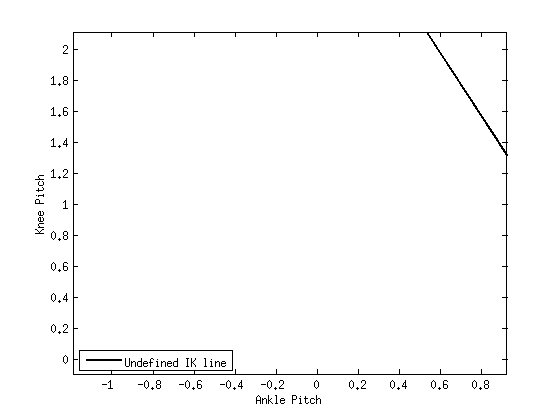
\includegraphics[height = 10cm]{Figures/locus.png}
 		\caption{Undefined Locus For Legs}
 		\label{fig:unlocus}
	\end{center}
\end{figure}

Now we can reconstruct and remove the rotation at the end and the transformation from ankle pitch to ankle roll from the chain to make it simpler
\[
T_{\text{llegRotated}'} = T_\text{llegRotated}\left(T^6_5R_z\left(\pi\right)R_y(-\tfrac{\pi}{2})\right)^{-1}
\]
\[
T_{\text{llegInv}'} = \left( T_{\text{llegRotated}'} \right) ^{-1}
\]
Now we have $p_x = T_{\text{llegInv}'(1,4)}$, $p_y = T_{\text{llegInv}'(2,4)}$ and $p_z = T_{\text{llegInv}'(3,4)}$. From the new symbolic transformation matrix we have:
\begin{align*}
&r_{14} = l_2\cos\theta_5 + l_1\left(\cos\theta_5\cos\theta_4 - \sin\theta_5\sin\theta_4\right)\\
&r_{24} = -l_2\sin\theta_5 - l_1\left(\sin\theta_5\cos\theta_4 + \cos\theta_5\sin\theta_4\right)\\
&r_{34} = 0
\end{align*}
We only need the translation part to extract $\theta_5$, so:
\begin{align*}
&\cos\theta_5\left(l_2+l_1\cos\theta_4\right) = p_x + l_2\sin\theta_5\sin\theta_4 & \Leftrightarrow\\
&\cos\theta_5 = \cfrac{p_x + l_1\sin\theta_5\sin\theta_4}{l_2+l_1\cos\theta_4}&\text{if }l_2+l_1\cos\theta_4\neq0\\
\end{align*}
The $l_2+l_1\cos\theta_4$ is zero if and only if $\cos\theta_4 = 1.029$. So it is always greater than zero, because $-1 \leq \cos \leq 1$:
\begin{align*}
&\sin\theta_5\left(-l_2-l_1\cos\theta_4\right) - l_2\cos\theta_5\sin\theta_4 = p_y& \Leftrightarrow\\
&\sin\theta_5\left(-l_2-l_1\cos\theta_4\right) - l_2\cfrac{p_x + l_1\sin\theta_5\sin\theta_4}{l_2+l_1\cos\theta_4}\sin\theta_4\ =p_y & \Leftrightarrow\\
&-\sin\theta_5\left(l_2+l_1\cos\theta_4\right) - \cfrac{l_2p_x\sin\theta_4}{l_2+l_1\cos\theta_4} - \cfrac{-{l_2}^2\sin\theta_5\sin^2\theta_4}{l_2+l_1\cos\theta_4} = p_y&\Leftrightarrow\\
&-\sin\theta_5\left(l_2+l_1\cos\theta_4\right)^2 - {l_2}^2\sin\theta_5\sin^2\theta_4 = p_y\left(l_2+l_1\cos\theta_4\right) + l_2p_x\sin\theta_4 & \Leftrightarrow\\
&\theta_5 = \arcsin\left(-\frac{p_y\left(l_2+l_1\cos\theta_4\right) + l_1p_x\sin\theta_4}{{l_1}^2\sin^2\theta_4 + \left(l_2 + l_1\cos\theta_4\right)}\right)
\end{align*}
We can do the division because ${l_1}^2\sin^2\theta_4 + \left(l_2 + l_1\cos\theta_4\right)^2$ is obviously greater than zero. 
Now we can remove the two transformations of $\theta_4$ and $\theta_5$ from the symbolic matrix and then we will have a transformation matrix that is a rotation matrix:
\[
T_{\text{llegRotated}''} = T_{\text{llegRotated}'}\left(T^4_3T^5_4\right)^{-1}
\]
\[
T_{\text{llegInv}''} = \left(T_{\text{llegRotated}''}\right)^{-1}
\]
And the rotation part is:
\begin{align*}
&r_{11} = \cos\widehat{\theta}_1\cos\widehat{\theta}_2\cos\theta_4 - \sin\widehat{\theta}_1\sin\theta_3\\
&r_{12} = -\cos\theta_3\sin\widehat{\theta}_1 - \cos\widehat{\theta}_1\cos\widehat{\theta}_2\sin\theta_3\\
&r_{13} = \cos\widehat{\theta}_1\sin\widehat{\theta}_2 \\
&r_{21} = -\cos\theta_3\sin\widehat{\theta}_2\\
&r_{22} = \sin\widehat{\theta}_2\sin\theta_3\\
&r_{23} = \cos\widehat{\theta}_2\\
&r_{31} = -\cos\widehat{\theta}_2\cos\theta_3\sin\widehat{\theta}_1 - \cos\widehat{\theta}_1\sin\theta_3\\
&r_{32} = -\cos\widehat{\theta}_1\cos\theta_3 + \cos\widehat{\theta}_2\sin\widehat{\theta}_1\sin\theta_3\\
&r_{33} = -\sin\widehat{\theta}_1\sin\widehat{\theta}_2
\end{align*}
Finally we can extract, from the transformation matrix, the remaining three angles:
\begin{align*}
\widehat{\theta}_2 &= \arccos T_{\text{llegInv}''(2,3)}\\
\theta_2 &= \widehat{\theta}_2 - \cfrac{\pi}{4}\\
\theta_3 &= \arcsin\left(\cfrac{T_{\text{llegInv}''(2,2)}}{\sin\left(\theta_2+\frac{\pi}{4}\right)}\right)\\
\widehat{\theta}_1 &= \arccos\left(\cfrac{T_{\text{llegInv}''(3,3)}}{\sin\left(\theta_2+\frac{\pi}{4}\right)}\right)\\
\theta_1 &= \widehat{\theta}_1 + \cfrac{\pi}{2}
\end{align*}
The equations above don't have any problem with division by zero because of the restriction of NAO. The HipRoll joint $(\theta_2)$ doesn't reach $-\frac{\pi}{4}$ or $\frac{3\pi}{4}$ so the denominator never becomes zero. Finally, we will do a forward validation step for all possible set of angles.
Below there are all the equations of inverse kinematics for the left leg:
\begin{align*}
T_\text{llegInv} &= \left(R_x(\tfrac{\pi}{4})\left(\left(A^0_\text{Base}\right)^{-1} T_\text{lleg} \left(A^\text{End}_6\right)^{-1}\right)\right)^{-1} \\
\theta_4 &=\pi - \arccos\left(\frac{{l_1}^2 + {l_2}^2 - \sqrt{\left(s_x-p_x\right)^2 + \left(s_y-p_y\right)^2 + \left(s_z-p_z\right)^2}^2}{2 l_1 l_2}\right) \\
\theta_6 &= \arctan\left(\frac{p_y}{p_z}\right)\hspace{3cm}\text{if} \left(l_2\cos\theta_5 + l_1 \cos\left(\theta_4 + \theta_5\right)\right) \neq 0 \\
T_{\text{llegInv}'} &= \left(\left(T_\text{llegInv}\right)^{-1}\left(T^6_5R_z\left(\pi\right)R_y(-\tfrac{\pi}{2})\right)^{-1}\right)^{-1} \\
\theta_5 &= \arcsin\left(-\frac{p_y\left(l_2+l_1\cos\theta_4\right) + l_1p_x\sin\theta_4}{{l_1}^2\sin^2\theta_4 + \left(l_2 + l_1\cos\theta_4\right)}\right) \\
\theta_5 &= \pi - \arcsin\left(-\frac{p_y\left(l_2+l_1\cos\theta_4\right) + l_1p_x\sin\theta_4}{{l_1}^2\sin^2\theta_4 + \left(l_2 + l_1\cos\theta_4\right)}\right)\\
T_{\text{llegInv}''} &= \left(\left(T_{\text{llegInv}'}\right)^{-1}\left(T^4_3T^5_4\right)^{-1}\right)^{-1} \\
\theta_2 &= \pm\arccos T_{\text{llegInv}''(2,3)} - \cfrac{\pi}{4} \\
\theta_3 &= \arcsin\left(\cfrac{T_{\text{llegInv}''(2,2)}}{\sin\left(\theta_2+\frac{\pi}{4}\right)}\right) \\
\theta_3 &= \pi - \arcsin\left(\cfrac{T_{\text{llegInv}''(2,2)}}{\sin\left(\theta_2+\frac{\pi}{4}\right)}\right) \\
\theta_1 &= \pm\arccos\left(\cfrac{T_{\text{llegInv}''(3,3)}}{\sin\left(\theta_2+\frac{\pi}{4}\right)}\right) + \cfrac{\pi}{2}
\end{align*}

\subsection{Inverse Kinematics for the Right Leg}
As we mentioned before, the chains of the legs are symmetric, so we will have a similar solution for the problem as we had with the arms. The only changes are in the rotation matrix that we use to rotate the HipYawPitch joint. Now we must rotate by $-\frac{\pi}{4}$.
\[
T_{\text{rleg}} = A^0_\text{Base}T^1_0T^2_1T^3_2T^4_3T^5_4T^6_5R_z(\pi)R_y(-\tfrac{\pi}{2})A^\text{End}_6
\]
\[
T_{\text{rleg}'} = T_\text{rleg}{\left(A^\text{End}_6\right)}^{-1}
\]
\[
T_{\text{rleg}''} = {\left(A^0_\text{Base}\right)}^{-1}T_{\text{rleg}'}
\]
\[
T_\text{rlegRotated} = R_x(-\tfrac{\pi}{4}) T_{\text{rleg}''}
\]
\[
T_\text{rlegInv} = {\left(T_\text{rlegRotated}\right)}^{-1}
\]
After that, the symbolic matrix for the right leg is exactly the same as the symbolic matrix for the left leg. From this point of view, if we follow all the steps as we did with the left leg, we will conclude to the same equations. So, the final equations are:
\begin{align*}
T_\text{rlegInv} &= \left(R_x(\tfrac{\pi}{4})\left(\left(A^0_\text{Base}\right)^{-1} T_\text{rleg} \left(A^\text{End}_6\right)^{-1}\right)\right)^{-1} \\
\theta_4 &=\pi - \arccos\left(\frac{{l_1}^2 + {l_2}^2 - \sqrt{\left(s_x-p_x\right)^2 + \left(s_y-p_y\right)^2 + \left(s_z-p_z\right)^2}^2}{2 l_1 l_2}\right) \\
\theta_6 &= \arctan\left(\frac{p_y}{p_z}\right)\hspace{3cm}\text{if} \left(l_2\cos\theta_5 + l_1 \cos\left(\theta_4 + \theta_5\right)\right) \neq 0 \\
T_{\text{rlegInv}'} &= \left(\left(T_\text{rlegInv}\right)^{-1}\left(T^6_5R_z\left(\pi\right)R_y(-\tfrac{\pi}{2})\right)^{-1}\right)^{-1} \\
\theta_5 &= \arcsin\left(-\frac{p_y\left(l_2+l_1\cos\theta_4\right) + l_1p_x\sin\theta_4}{{l_1}^2\sin^2\theta_4 + \left(l_2 + l_1\cos\theta_4\right)}\right) \\
\theta_5 &= \pi - \arcsin\left(-\frac{p_y\left(l_2+l_1\cos\theta_4\right) + l_1p_x\sin\theta_4}{{l_1}^2\sin^2\theta_4 + \left(l_2 + l_1\cos\theta_4\right)}\right)\\
T_{\text{rlegInv}''} &= \left(\left(T_{\text{rlegInv}'}\right)^{-1}\left(T^4_3T^5_4\right)^{-1}\right)^{-1} \\
\theta_2 &= \pm\arccos T_{\text{rlegInv}''(2,3)} + \cfrac{\pi}{4} \\
\theta_3 &= \arcsin\left(\cfrac{T_{\text{rlegInv}''(2,2)}}{\sin\left(\theta_2 - \frac{\pi}{4}\right)}\right) \\
\theta_3 &= \pi - \arcsin\left(\cfrac{T_{\text{rlegInv}''(2,2)}}{\sin\left(\theta_2 - \frac{\pi}{4}\right)}\right) \\
\theta_1 &= \pm\arccos\left(\cfrac{T_{\text{rlegInv}''(3,3)}}{\sin\left(\theta_2 - \frac{\pi}{4}\right)}\right) + \cfrac{\pi}{2}
\end{align*}

\subsection{Undefined Target Points For Legs}
\label{undefined}
As we mentioned before, we have some target points for which we can't find an inverse kinematics solution. These target points are presented in the figure~\ref{fig:undefined}, alongside with all the values of the angles that are responsible for this singularity. As we can see, we let the robot to do a lot of movements in the field, and none of those movements was close to the points of the singularity. In real world, it is very rare for someone to give target points in that area. Also, when someone is executing a trajectory, they ''feed'' inverse kinematics with a lot of target points per second (usually they provide inverse kinematics with target points with frequency 50 to 100 Hz), so if one of those target points is in the area of singularity, we will find a solution for the next target point. Because we are working in high frequency rate, the singularity will be unnoticed and the movement will be continued normally.

\begin{figure}[h]
	\begin{center}
		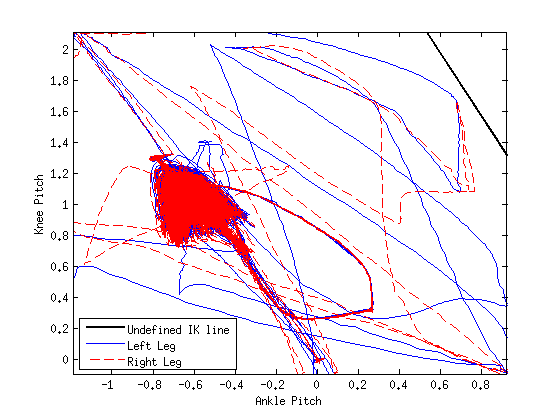
\includegraphics[height = 10cm]{Figures/undefined.png}
 		\caption{Undefined Target Points For Legs}
 		\label{fig:undefined}
	\end{center}
\end{figure}


\section{Implementation}
Now that we have all the equations for both problems, we must integrate them in the code of the team. The code of the team is written in \verb!C++! so because \verb!C++! doesn't have any library for fast linear algebra operations, we must develop a minimalistic matrix framework. Then, using this framework, we must write some functions that will implement the equations of forward and inverse kinematics in \verb!C++!.

\subsection{KMat: Kouretes Math Library}
KMat is a library developed by Emmanouil Orfanoudakis~\cite{orfanoudakis2011} that supports a strict subset of algebraic operations. The focus of the library is mainly in real numbers operations and the primary goal of KMat is low memory footprint and calculation efficiency. The typical linear algebra libraries do run-time validation for the compatibility of the operands and are optimized for large matrices. On the other hand, KMat is optimized for small matrices (typically $(3\times3)$ or $(4\times4)$) and only a subset of operations (addition, subtraction, multiplication, scalar addition, scalar multiplication, transposition, inversion) have been implemented. KMat supports two type of matrices: Dense matrices and Affine transformation matrices.

For our work we used mainly the affine type of matrices and we expanded the functions of the library with some functions that are extremely useful for the kinematics computations. These functions are some initialization functions that initialize a matrix with the given DH parameters or reconstruct of the matrix given the target points etc.

\subsection{Nao Kinematics in C++}
Along with KMat we created two more libraries ForwardKinematics and InverseKinematics. ForwardKinematics has the functions to calculate the location of an end effector of a kinematic chain, given the joint values for this chain. The union of independent chains with common base frame is possible, so someone can take the position of the top camera relatively to one of the legs. Finally, we have a function to calculate the center of mass of the robot. The input of each function is the values of the joints with the order that they appear in the kinematic chains.

The inverse kinematics library has five functions, each of which solves the problem for a kinematic chain. All functions take, as input, the position and the orientation of the target point and the output is the values of the joints, for all the possible solutions for this point. It is possible to have a solution with two set of values and then the user can decide what output will be used. 

As we mentioned before, the legs have one common joint (HipYawPitch) but if we give two target points, one for each leg, inverse kinematics for the left leg will most likely  return a different value for this joint than the inverse kinematics for the right leg. We must decide what value will be set to the HipYawPitch joint and one solution to this problem is to make the support leg (the leg that keeps the robot in balance) the master of this joint or another solution is to get the mean of these two values. Both solutions are not perfect but with a large probability, if we design trajectories carefully, the resulted values from inverse kinematics for this joint will be close enough. Thus, we can use any of these two solutions and the result will be similar to the result if the joint was independent.
 \chapter{Results}
\label{Results}
We have a lot of ways to check if solutions for both problems are working correctly. The testing for forward kinematics is trivial; we just move the end effector to a position and we just check if forward kinematics returned the correct position and orientation. On the other hand, the testing of inverse kinematics was more difficult because we must give a valid target point if we want inverse kinematics to return a solution.

The problem is that we don't know the work space for the end effectors of NAO. So, we came up with another way to validate our solution. We moved one end effector to a random position, then we took the position and the orientation of this point from forward kinematics and then we assigned this point as the target point for inverse kinematics. Then we checked if inverse kinematics found a solution and we know that the solution inverse kinematics returned is correct, because there is a step of forward kinematics inside inverse kinematics that validates the output.

We made two demos to present kinematics in real world. The first demo tests inverse kinematics of the arm along with forward kinematics of the legs. The second demo is more complicated and checks inverse kinematics of the legs and the calculation of the center of mass.


\section{Real Time Performance}
In table~\ref{times} we can see the execution times for each function (of inverse kinematics) in microseconds (us). Unfortunately, we can't compare these times with the Aldebaran's solution execution time, because it is not independent and along with the solution for inverse kinematics, it does the movement of the joints of the chain. So, we can't extract ``clean'' times from the execution.

\begin{table}[!h]
\centering
\caption{Execution Times}
\vspace*{0.06cm}
\begin{tabular}{|l|c|}
\hline
\textbf{Function} & \textbf{Time (us)}\\ \hline
Forward For Head & 59.43 \\
Forward For Left Arm & 75.94 \\
Forward For Right Arm & 79.72 \\
Forward For Left Leg & 94.58 \\
Forward For Right Leg & 95.16 \\
Inverse For Head & 82.04 \\
Inverse For Left Arm & 205.91 \\
Inverse For Right Arm & 214.56 \\
Inverse For Left Leg & 203.32 \\
Inverse For Right Leg & 152.62 \\
Calculation of CoM & 410.30 \\
\hline
\end{tabular}
\label{times}
\end{table}

\section{Pointing To The Ball}
In the first demo we want to make NAO point to the ball with the hands. We used, along with the kinematics, the vision~\cite{orfanoudakis2011} and the world state model of the robot. First, NAO searches for the ball and when it finds it, NAO points to the ball with one or two hands. With the help of the world state model, if NAO loses the ball, it can continue to point to the area that the ball must be according to the last vision observations.

The ball observation can be described as a two-dimensional point without orientation. The coordination of the ball is described as polar coordinates, so we have the distance and the angle of the observation relatively to the projection of the torso on the floor. We must now move this point from two-dimensions to three-dimensions and give it an orientation. First, we transform the polar coordinates to Cartesian coordinates ($ p_x,p_y $) and we add the height of the torso as the \(p_z\). Now we know the position in the three-dimensional space and we also know that \(a_x\) equals to zero because we are only rotating \(y\)-axis (up/down) and \(z\)-axis (right/left). To find the two other angles, we get the straight line that connects the point of the ball and the position of the shoulder pitch joint relatively to the torso frame. Then we have that \(a_y\) equals to the angle between this line and the \(y\)-axis and similarly we find the \(a_z\). Now we must calculate the position of the target point, which is in the line and from a distance \(d\) from the joint, where \(d\) is the size of the stretched arm (this is the maximum size of the arm). We need to bring the target point to that distance, because only then it will be a valid target point for inverse kinematics. We do this operation two times, one for each arm (different position of the shoulder joint) and then we give to inverse kinematics for left and right arm the resulted target points. Below there are images from the demo:
\begin{figure}[!h]
\centerline{
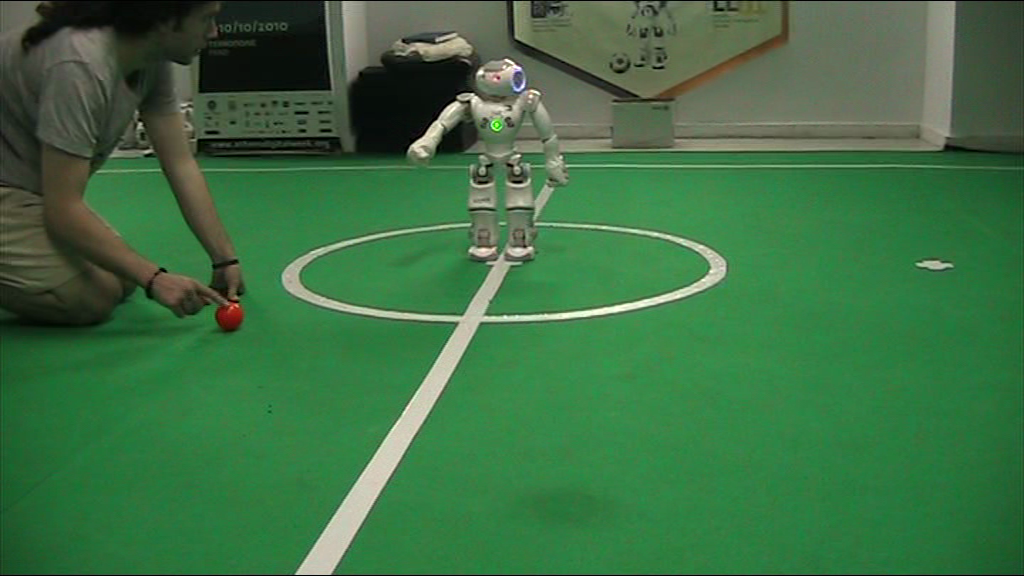
\includegraphics[width=0.32\textwidth]{Figures/Demo1/1.png}
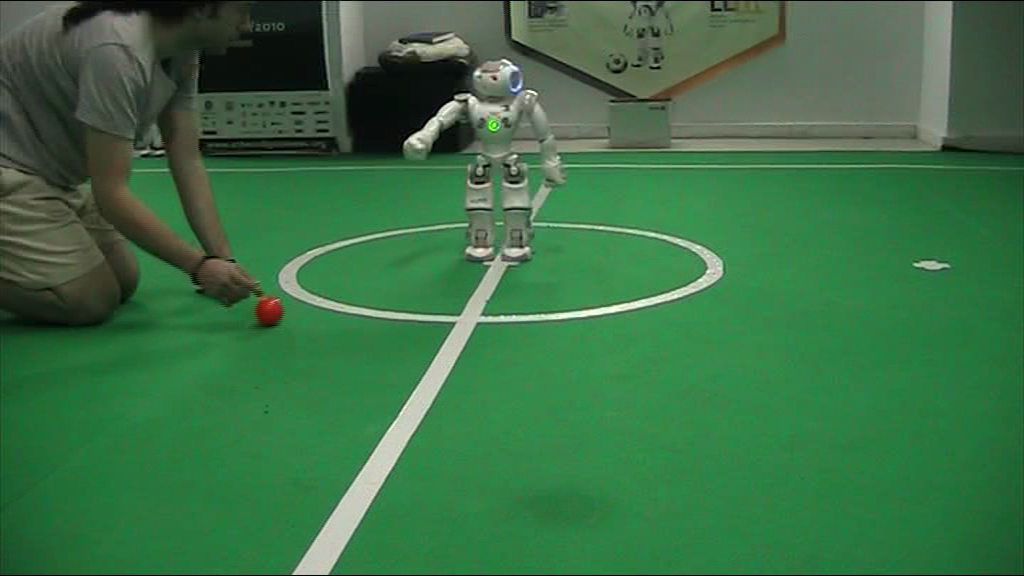
\includegraphics[width=0.32\textwidth]{Figures/Demo1/2.png}
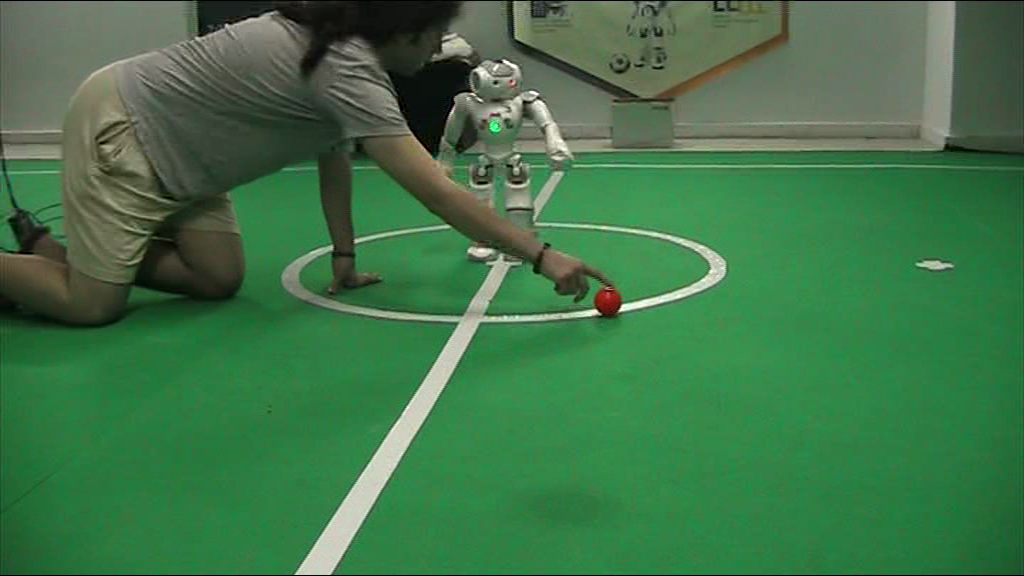
\includegraphics[width=0.32\textwidth]{Figures/Demo1/3.png}
}
\vspace*{0.06cm}
\centerline{
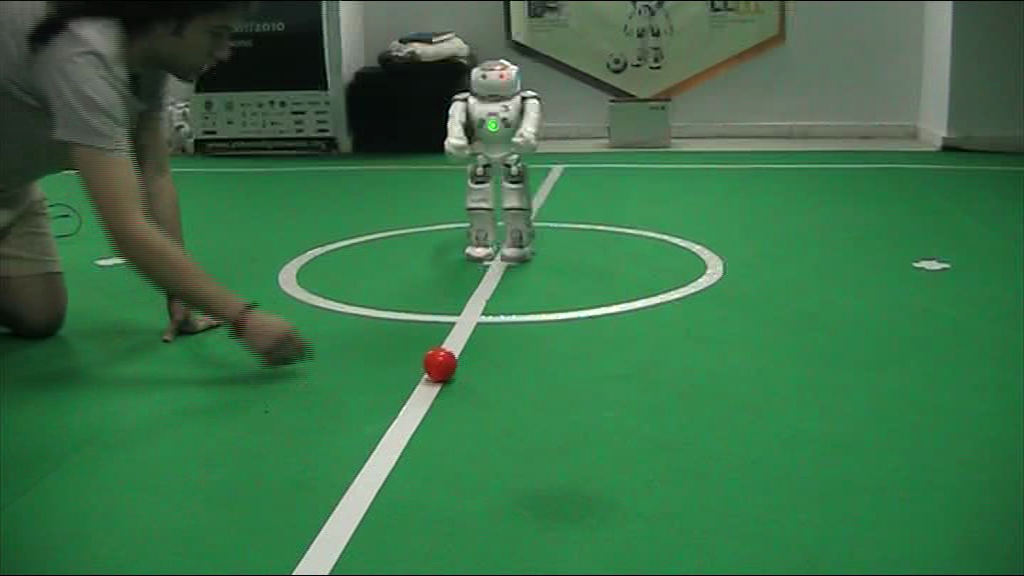
\includegraphics[width=0.32\textwidth]{Figures/Demo1/4.png}
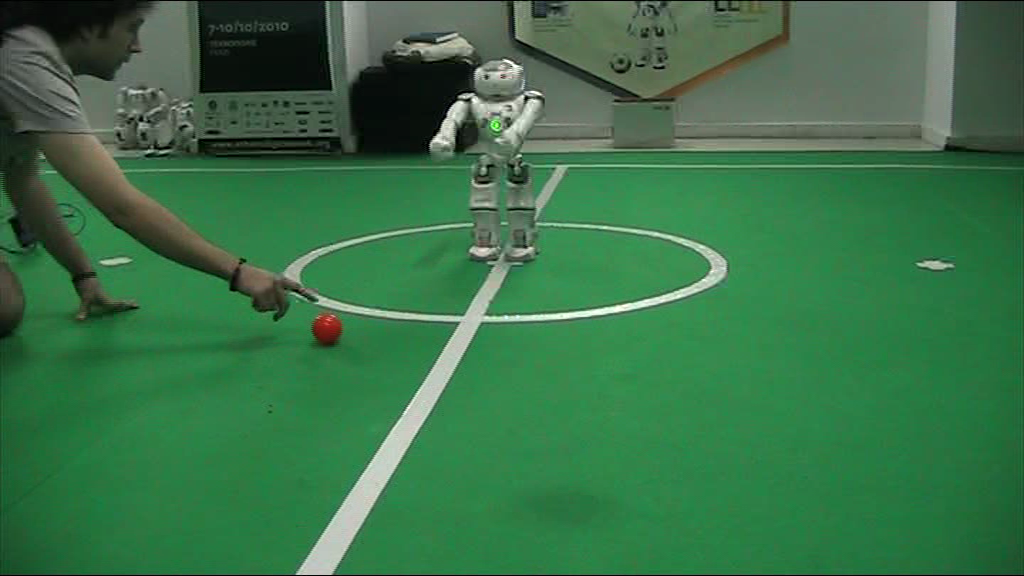
\includegraphics[width=0.32\textwidth]{Figures/Demo1/5.png}
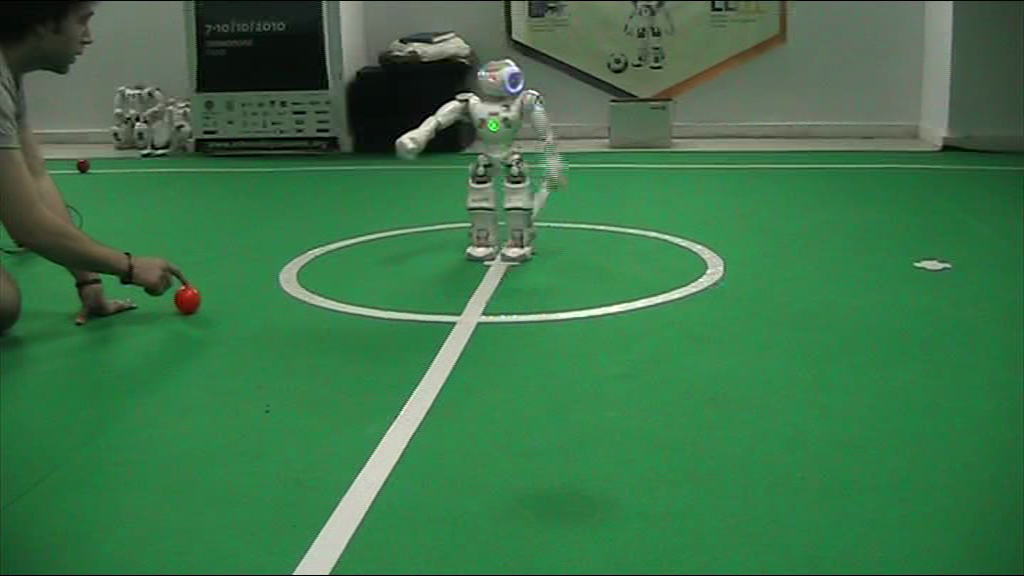
\includegraphics[width=0.32\textwidth]{Figures/Demo1/6.png}
}
\vspace{-0.1cm}
\caption{Point the ball using forward and inverse kinematics}
\label{demo1}
\vspace*{0.5cm}
\end{figure}
\section{Balancing Using The Center of Mass}

In the second demo we want to make NAO to move one of its legs to the point of the projection of the CoM on the floor, so, we will have a very basic balancing system. First of all, we must calculate the position of the CoM using forward kinematics. Now we have the CoM position relatively to the torso frame. The problem is that the torso frame is never parallel to the floor. Thus, we get from the gyro-meters the angleX and angleY of the torso plain. Now we can take the position of the CoM relatively to the rotated torso:

\[
	T_{\text{rotated}} = R_y(\text{angleY})R_x(\text{angleX})A_{\text{CoM}}
\]

Then we put a custom value to \(p_z\) which represents the desired torso height from the floor, so, now we have \(T_{\text{rotated}'}\). Now we must rotate back to the torso frame, so:

\[
	T_{\text{final}} = \left(R_y(\text{angleY})R_x(\text{angleX})\right)^{-1}T_{\text{rotated}'}
\]

Finally, we set  \(p_x\), \(p_y\) and \(p_z\) from \(T_{\text{final}}\) as the target point for inverse kinematics and we set \(a_x = -\)angleX, \(a_y = -\)angleY and \(a_z = 0\) as the target rotation, because we don't care about rotation around \(z\)-axis. Now the target point is the projection of the CoM to the floor and the rotation of the end effector is parallel to the frame of the floor.

In the figures below we can see that the foot is always parallel to the floor. It happens some times, that some robots have displaced inertial unit (accelerometers and gyro-meters). On these robots we can see that the foot is not parallel to the floor but this is a hardware problem and not a kinematics problem.

\begin{figure}[!h]
\centerline{
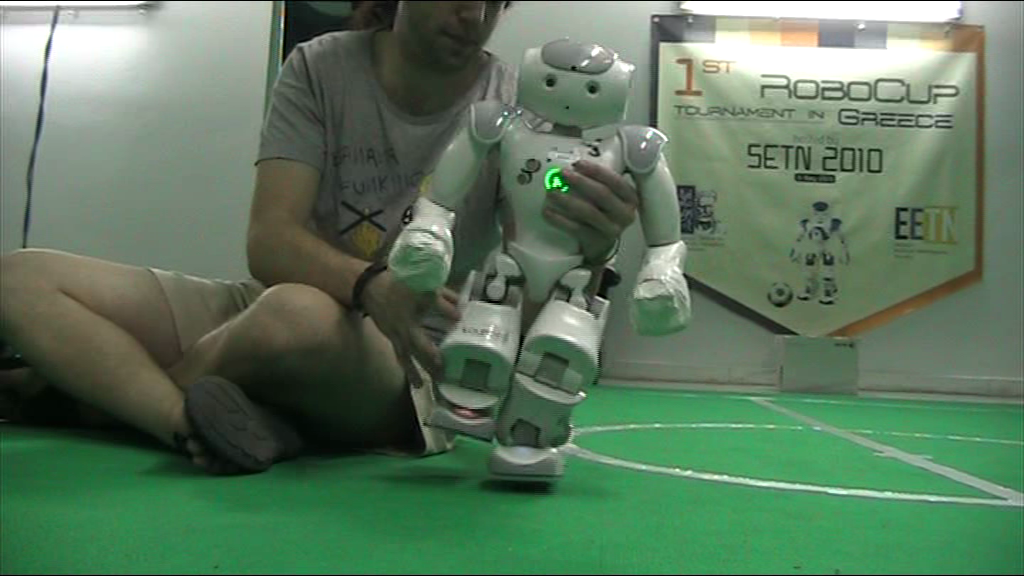
\includegraphics[width=0.32\textwidth]{Figures/Demo2/1.png}
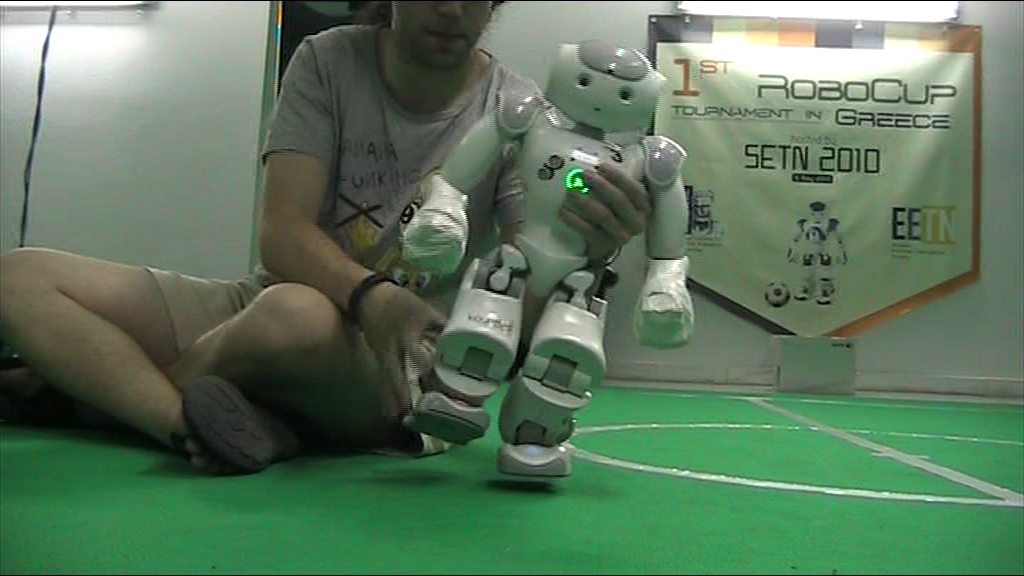
\includegraphics[width=0.32\textwidth]{Figures/Demo2/2.png}
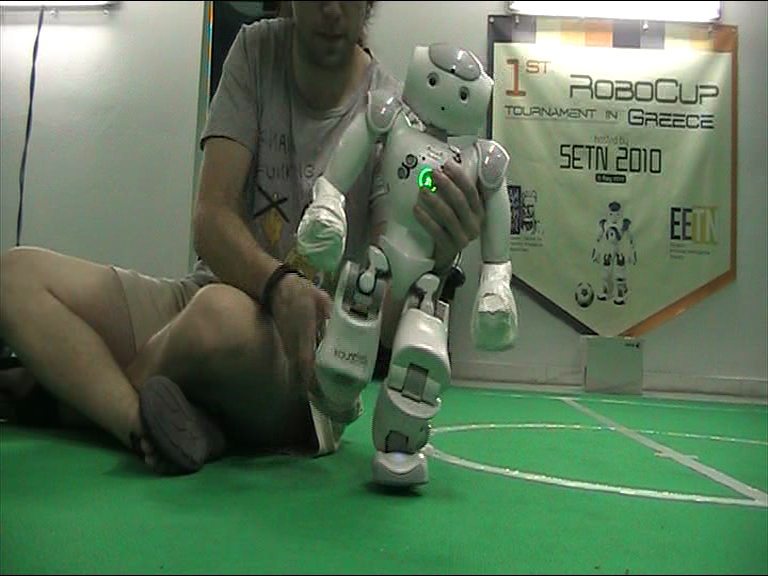
\includegraphics[width=0.32\textwidth]{Figures/Demo2/3.png}
}
\vspace*{0.06cm}
\centerline{
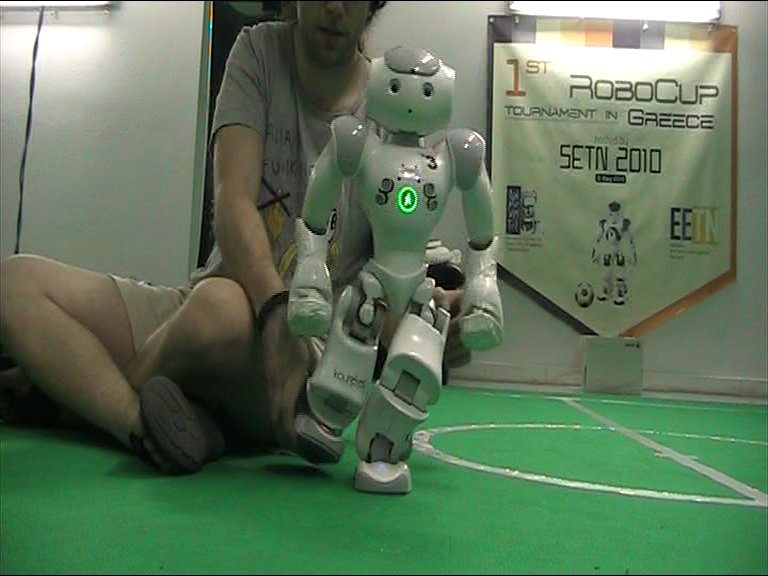
\includegraphics[width=0.32\textwidth]{Figures/Demo2/4.png}
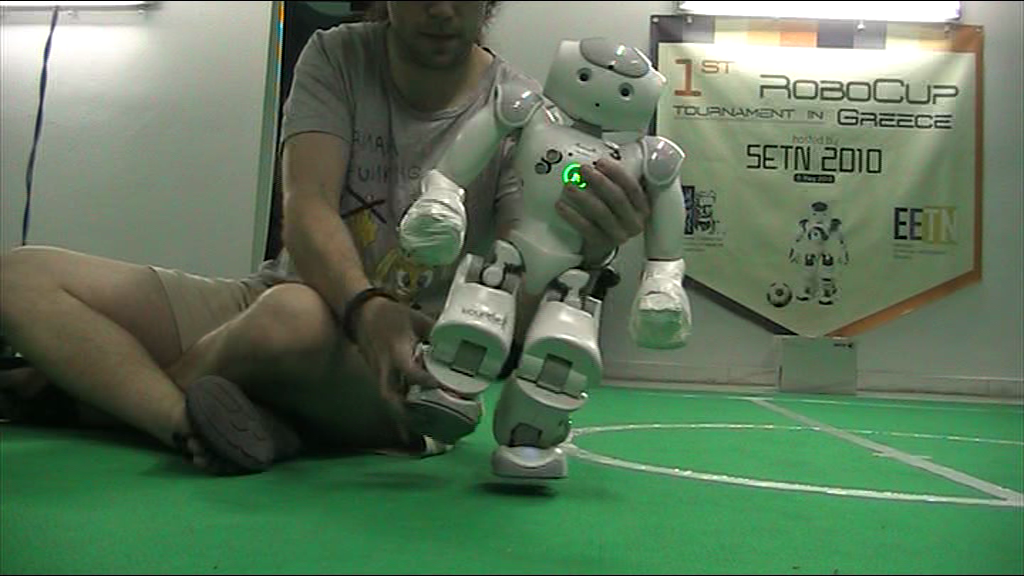
\includegraphics[width=0.32\textwidth]{Figures/Demo2/5.png}
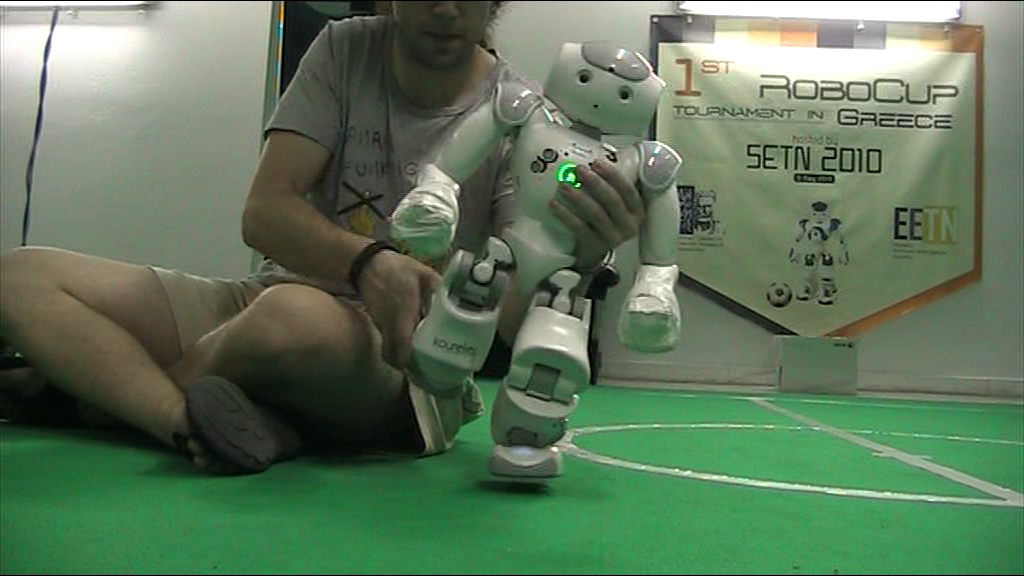
\includegraphics[width=0.32\textwidth]{Figures/Demo2/6.png}
}
\vspace{-0.1cm}
\caption{Basic balance system using center of mass}
\label{demo1}
\vspace*{0.5cm}
\end{figure}

 \chapter{Conclusion}
\label{conclusion}

Kinematics is the base for several applications related to robot motion. Our approach to NAO kinematics is based on standard principled methods for studying robot kinematic chains. Nevertheless, no complete analytical solution for the NAO robot had been published before. Our work offers such a complete analytical solution, which we expect will be useful not only to RoboCup SPL teams, but also to any NAO software developer. 


\section{Future Work}
The work in this thesis can be used as the base for a several future research directions, some of which are listed below. It is also a step towards making the software architecture of our team independent from Aldebaran's development framework.

\subsubsection*{Omni-Directional Walk}

The ability of a robot to walk towards any desired direction is called omni-directional walk. The feet (and arms) trajectories in omni-directional walk engines are being calculated dynamically and for this reason an inverse kinematics mechanism is more than necessary for the robot to be able to follow them. 

\subsubsection*{Dynamic Balancing}

As the robot walks, kicks, or performs any kind of motion, it must maintain its balance. Knowledge of the position of the center of mass at all times is more than necessary for successful balancing.

\subsubsection*{Kick Engine}

Currently, our team relies  only on static predefined kicks designed. The problem with those kicks is that they cannot absorb random disturbances and quite often robots executing them fall down. With inverse kinematics and balancing in place, the team can develop a dynamic kick engine, which takes care of balancing the robot on one leg, while following a dynamic kick trajectory based on the ball's position with the other leg.



\bibliographystyle{StyleFiles/splncs}
\renewcommand{\bibname}{References} % changes default name Bibliography to References
\bibliography{thesis}
\addcontentsline{toc}{chapter}{References} %adds References to contents page


\end{document}